\documentclass[
]{jss}

%% recommended packages
\usepackage{orcidlink,thumbpdf,lmodern}

\usepackage[utf8]{inputenc}

\author{
Fabien Girka~\orcidlink{0000-0003-2843-1104}\\Laboratoire des Signaux et
Systèmes \And Etienne Camenen\\INSERM \And Caroline Peltier\\INRAE
\AND Arnaud Gloaguen\\CEA \And Vincent Guillemot\\Institut Pasteur
\AND Laurent Le Brusquet\\Laboratoire des Signaux et
Systèmes \And Arthur
Tenenhaus~\orcidlink{0000-0003-3459-1518}\\Laboratoire des Signaux et
Systèmes
}
\title{Multiblock data analysis with the RGCCA package}

\Plainauthor{Fabien Girka, Etienne Camenen, Caroline Peltier, Arnaud
Gloaguen, Vincent Guillemot, Laurent Le Brusquet, Arthur Tenenhaus}
\Plaintitle{Multiblock data analysis with the RGCCA package}
\Shorttitle{Regularized Generalized Canonical Correlation Analysis}


\Abstract{
Multiblock component methods aim to study the relationships between
several sets of variables. Regularized Generalized Canonical Correlation
Analysis (RGCCA) is a unified and flexible framework that gathers fifty
years of multiblock component methods. RGCCA offers a unified
implementation strategy for all these methods. This implementation is
made available within the RGCCA package. In addition, the RGCCA package
produces graphical outputs and statistics to assess the
robustness/significance of the analysis. The usefulness of the RGCCA
package is illustrated in this paper on two real datasets. The RGCCA
package is freely available on the ComprehensiveR Archive Network (CRAN)
\url{http://www.r-project.org/} and GitHub
\url{https://github.com/rgcca-factory/RGCCA}.
}

\Keywords{Multiblock component methods, RGCCA, data integration}
\Plainkeywords{Multiblock component methods, RGCCA, data integration}

%% publication information
%% \Volume{50}
%% \Issue{9}
%% \Month{June}
%% \Year{2012}
%% \Submitdate{}
%% \Acceptdate{2012-06-04}

\Address{
    Fabien Girka\\
    Laboratoire des Signaux et Systèmes\\
    Université Paris-Saclay, CNRS, CentraleSupélec,
\newline  Gif-sur-Yvette, 91190, France \newline Institut du Cerveau de
Paris (ICM), Sorbonne Université \newline  Assistance Publique-Hôpitaux
de Paris (AP-HP)\\
  E-mail: \email{fabien.girka@centralesupelec.fr}\\
  
      Etienne Camenen\\
    INSERM\\
    Inserm U1127, CNRS UMR 7225, \newline Hôpital Universitaire
Pitié-Salpêtrière \newline  75013 Paris, France \newline Institut du
Cerveau de Paris (ICM), Sorbonne Université \newline  Assistance
Publique-Hôpitaux de Paris (AP-HP)\\
  
  
      Caroline Peltier\\
    INRAE\\
    Centre des Sciences du Goût et de l'Alimentation \newline CNRS,
INRAE, Institut Agro \newline University of Bourgogne F-21000 Dijon
\newline CNRS, INRAE, PROBE research infrastructure \newline  ChemoSens
facility, F-21000 Dijon, France \newline Institut du Cerveau de Paris
(ICM), Sorbonne Université \newline  Assistance Publique-Hôpitaux de
Paris (AP-HP)\\
  
  
      Arnaud Gloaguen\\
    CEA\\
    Centre National de Recherche en Génomique Humaine \newline  Institut
de Biologie François Jacob \newline  CEA, Université Paris-Saclay, Évry,
France\\
  
  
      Vincent Guillemot\\
    Institut Pasteur\\
    Université Paris Cité \newline Bioinformatics and Biostatistics Hub
\newline  F-75015 Paris, France\\
  
  
      Laurent Le Brusquet\\
    Laboratoire des Signaux et Systèmes\\
    Université Paris-Saclay, CNRS, CentraleSupélec
\newline  Gif-sur-Yvette, 91190, France\\
  
  
      Arthur Tenenhaus\\
    Laboratoire des Signaux et Systèmes\\
    Université Paris-Saclay, CNRS, CentraleSupélec
\newline  Gif-sur-Yvette, 91190, France \newline Institut du Cerveau de
Paris (ICM), Sorbonne Université \newline  Assistance Publique-Hôpitaux
de Paris (AP-HP)\\
  E-mail: \email{arthur.tenenhaus@centralesupelec.fr}\\
  
  }


% tightlist command for lists without linebreak
\providecommand{\tightlist}{%
  \setlength{\itemsep}{0pt}\setlength{\parskip}{0pt}}

% From pandoc table feature
\usepackage{longtable,booktabs,array}
\usepackage{calc} % for calculating minipage widths
% Correct order of tables after \paragraph or \subparagraph
\usepackage{etoolbox}
\makeatletter
\patchcmd\longtable{\par}{\if@noskipsec\mbox{}\fi\par}{}{}
\makeatother
% Allow footnotes in longtable head/foot
\IfFileExists{footnotehyper.sty}{\usepackage{footnotehyper}}{\usepackage{footnote}}
\makesavenoteenv{longtable}



\usepackage{amsmath} \usepackage{amsfonts} \usepackage{times} \usepackage{bm} \usepackage{soul} \usepackage{epsfig} \usepackage{amssymb} \usepackage{lscape} \usepackage{float} \usepackage{latexsym} \usepackage{graphicx,psfrag,color} \usepackage{multirow}  \usepackage[space]{grffile} \usepackage{amsthm} \usepackage{enumerate} \usepackage{enumitem} \usepackage{setspace} \usepackage{subfigure} \usepackage{longtable} \usepackage{etoolbox}  \usepackage{pdfpages} \usepackage[mathscr]{euscript} \usepackage[T1]{fontenc} \usepackage[misc]{ifsym} \usepackage{wasysym} \usepackage{hyperref} \usepackage[width=\textwidth]{caption} \usepackage{algorithmic, algorithm}

\begin{document}



\newtheorem{theorem}{theorem}[section]%
\newtheorem{lemma}[theorem]{Lemma}
\newtheorem{proposition}[theorem]{Proposition}
\newtheorem{corollary}[theorem]{Corollary}
\newtheorem{remark}[theorem]{Remark}

\hypertarget{introduction}{%
\section{Introduction}\label{introduction}}

A challenging problem in multivariate statistics is to study
relationships between several sets of variables measured on the same set
of individuals. This paradigm is referred to by several names, including
``learning from multimodal data'', ``data integration'', ``multiview
data'', ``multisource data'', ``data fusion'' or ``multiblock data
analysis''. Despite the availability of various statistical methods and
dedicated software for multiblock data analysis, handling multiple
highly multivariate datasets remains a critical issue for effective
analysis and knowledge discovery.

For the statistical computing environment R \cite{R2022}, various R
packages are available for multiblock data analysis. Four mainstream
references are \(\small{\texttt{mixOmics}}\) \cite{Rohart2017},
\(\small{\texttt{multiblock}}\) \cite{Liland2022},
\(\small{\texttt{ade4}}\) (\cite{Dray2007}), and
\(\small{\texttt{FactoMineR}}\) \cite{Le2008}. Each package uses its own
way of specifying multiblock models and storing the results.

Regularized Generalized Canonical Correlation Analysis (RGCCA) is a
unified statistical framework that subsumes, as special cases, an
astonishingly large number of multiblock component methods. RGCCA relies
on a single optimization problem with immediate practical consequences
for a unified statistical analysis and implementation strategy. In this
paper, we introduce an R package called \(\small{\texttt{RGCCA}}\)
(Girka et al, 2023), which implements the RGCCA framework.

Within the \(\small{\texttt{RGCCA}}\) package, all implemented methods
share the same function interface and a clear class structure. In
addition, \(\small{\texttt{RGCCA}}\) package relies on the single
\(\small{\texttt{rgcca()}}\) function for specifying the multiblock
models. It also provides several utility functions for data
preprocessing and several plots for diagnostics or visualization of the
results from multiblock analysis.\\
In addition, the package includes several built-in datasets and examples
to help users get started quickly. Package \(\small{\texttt{RGCCA}}\) is
available from the Comprehensive R Archive Network (CRAN), at
\url{https://CRAN.R-project.org/package=RGCCA} and can be installed from
the R console with the following command:

\footnotesize

\begin{CodeChunk}
\begin{CodeInput}
R> install.packages("RGCCA")
\end{CodeInput}
\end{CodeChunk}

\normalsize

In this paper, we present an overview of the RGCCA framework's
theoretical foundations, summarize the optimization problem under which
all the algorithms were designed, and provide code examples to
illustrate the package's usefulness and versatility. We believe that our
package provides a valuable contribution to the field of multiblock data
analysis and will enable researchers to conduct more effective analyses
and gain new insights into complex datasets.

The paper's remaining sections are organized as follows: Section 2
presents the general optimization problem. Section 3 summarizes the
theoretical foundations of the RGCCA framework
\cite{Tenenhaus2011, Tenenhaus2014, Tenenhaus2015, 
Tenenhaus2017}. Sections 4 and 5 provide code examples to illustrate the
package's capabilities. Finally, we conclude the paper in Section 6.

\hypertarget{optimization-background}{%
\section{Optimization background}\label{optimization-background}}

This section presents the optimization framework under which all the
algorithms proposed in the RGCCA framework were designed. The RGCCA
framework gathers several methods already presented in
\cite{Tenenhaus2011, Tenenhaus2014, Tenenhaus2015, Tenenhaus2017}. It is
recalled here for a broader class of constraints.

The RGCCA framework relies on a master algorithm for maximizing a
continuously differentiable multi-convex function
\(f( \mathbf a_1, \ldots, \mathbf a_J):\mathbb{R}^{p_1}\times \ldots \times \mathbb{R}^{p_J} \xrightarrow{}\mathbb{R}\)
(i.e.~for each \(j\), \(f\) is a convex function of \(\mathbf a_j\)
while all the other \(\mathbf a_k\) are fixed) under the constraint that
each \(\mathbf a_j\) belongs to a compact set
\(\Omega_j\subset \mathbb{R}^{p_j}\). This general optimization problem
can be formulated as follows:

\begin{align}
\underset{ \mathbf a_1, \ldots, \mathbf a_J}{\text{max}} f( \mathbf a_1, \ldots, \mathbf a_J)
\text{ s.t. }  \mathbf a_j \in \Omega_j, \text{ } j = 1, \ldots, J.
\label{master_optim}
\end{align}

For such a function defined over a set of parameter vectors
\(( \mathbf a_1, \ldots, \mathbf a_J)\), we make no difference between
the notations \(f( \mathbf a_1, \ldots, \mathbf a_J)\) and
\(f( \mathbf a)\), where \(\mathbf a\) is the column vector
\(\mathbf a = \left( \mathbf a_1^\top, \ldots, \mathbf a_J^\top\right)^\top\)
of size \(p = \sum_{j=1}^{J}p_j\). Moreover, the vertical concatenation
of a column vector is denoted
\(\mathbf a = \left( \mathbf a_1; \ldots; \mathbf a_J \right)\) for the
sake of simplification of notation.

\hypertarget{algorithm}{%
\subsection{Algorithm}\label{algorithm}}

A simple, monotonically, and globally convergent algorithm is presented
for solving optimization problem (\ref{master_optim}). The maximization
of the function \(f\) defined over different parameter vectors
(\(\mathbf a_1, \ldots, \mathbf a_J\)) is approached by updating each of
the parameter vectors in turn, keeping the others fixed. This update
rule was recommended in \cite{DeLeeuw1994} and is called Block
Relaxation or cyclic Block Coordinate Ascent (BCA).

Let \(\nabla_j f( \mathbf a)\) be the partial gradient of
\(f( \mathbf a)\) with respect to \(\mathbf a_j\). We assume
\(\nabla_j f( \mathbf a) \neq \mathbf{0}\) in this manuscript. This
assumption is not too binding as \(\nabla_j f( \mathbf a) = \mathbf{0}\)
characterizes the global minimum of
\(f( \mathbf a_1 , \ldots , \mathbf a_J )\) with respect to
\(\mathbf a_j\) when the other vectors
\(\mathbf a_1 , \ldots , \mathbf a_{j-1} , \mathbf a_{j+1} , \ldots , \mathbf a_J\)
are fixed.

We want to find an update \(\hat{ \mathbf a}_j\in \Omega_j\) such that
\(f( \mathbf a)\leq f( \mathbf a_1, ..., \mathbf a_{j-1}, \hat{ \mathbf a}_j, \mathbf a_{j+1}, ..., \mathbf a_J)\).
As \(f\) is a continuously differentiable multi-convex function and
considering that a convex function lies above its linear approximation
at \(\mathbf a_j\) for any \(\tilde{ \mathbf a}_j\in\Omega_j\), the
following inequality holds:

\begin{equation}
\begin{gathered}
f( \mathbf a_1, ...,  \mathbf a_{j-1}, \tilde{ \mathbf a}_j,  \mathbf a_{j+1}, \ldots,  \mathbf a_J) \geq f( \mathbf a) + \nabla_jf( \mathbf a)^\top(\tilde{ \mathbf a}_j -  \mathbf a_j).
\label{minorizing_ineq}
\end{gathered}
\end{equation}

On the right-hand side of the inequality (\ref{minorizing_ineq}), only
the term \(\nabla_jf( \mathbf a)^\top\tilde{ \mathbf a}_j\) is relevant
to \(\tilde{ \mathbf a}_j\) and the solution that maximizes the
minorizing function over \(\tilde{ \mathbf a}_j\in\Omega_j\) is obtained
by considering the following optimization problem:

\begin{equation}
\hat{ \mathbf a}_j = \underset{\tilde{ \mathbf a}_j\in\Omega_j}{\text{argmax }} \nabla_j f( \mathbf a)^\top \tilde{ \mathbf a}_j := r_j( \mathbf a).
\label{core_update}
\end{equation}

The entire algorithm is subsumed in Algorithm \ref{master_algo}.

\begin{algorithm}[!ht]
    \caption{Algorithm for the maximization of a continuously differentiable multi-convex function}
    \begin{algorithmic}[1]
        \STATE {\bfseries Result:} {$\mathbf a_1^s, \ldots,  \mathbf a_J^s$ (approximate solution of (\ref{master_optim}))}
        \STATE {\bfseries Initialization:} {choose random vector $\mathbf a_j^0\in\Omega_j, j =1, \ldots, J$, $\varepsilon$;}
        \STATE$s = 0$ ;
        \REPEAT
        \FOR{$j=1$ {\bfseries to} $J$}
        \STATE \hspace{-2cm}$\vcenter{\begin{equation}
             \mathbf a_j^{s+1} = r_j\left(  \mathbf a_1^{s+1}, \ldots,  \mathbf a_{j-1}^{s+1},  \mathbf a_j^{s}, \ldots,  \mathbf a_J^{s}\right).
        \end{equation}}$
        \ENDFOR
        \STATE$s = s + 1$ ;
        \UNTIL{$f( \mathbf a_1^{s+1}, \ldots,  \mathbf a_J^{s+1})-f( \mathbf a_1^s, \ldots,  \mathbf a_J^s) < \varepsilon$}
    \end{algorithmic}
    \label{master_algo}
\end{algorithm}

We need to introduce some extra notations to present the convergence
properties of Algorithm \ref{master_optim}:
\(\Omega = \Omega_1 \times \ldots \times \Omega_J\),
\(\mathbf a = \left( \mathbf a_1; \ldots; \mathbf a_J\right) \in \Omega\),
\(c_j \text{ : } \Omega\mapsto\Omega\) is an operator defined as
\(c_j( \mathbf a) = \left( \mathbf a_1; \ldots; \mathbf a_{j-1} ; r_j( \mathbf a) ; \mathbf a_{j+1} ; \ldots; \mathbf a_J\right)\)
with \(r_j( \mathbf a)\) introduced in equation (\ref{core_update}) and
\(c \text{ : } \Omega\mapsto\Omega\) is defined as
\(c = c_J\circ c_{J-1}\circ ... \circ c_1\), where \(\circ\) stands for
the composition operator. Using the operator \(c\), the
\guillemotleft for loop\guillemotright{} inside Algorithm
\ref{master_optim} can be replaced by the following recurrence relation:
\(\mathbf a^{s+1} = c( \mathbf a^s)\). The convergence properties of
Algorithm \ref{master_optim} are summarized in the following
proposition:

\begin{proposition}
    Let $\left\lbrace  \mathbf a^s\right\rbrace_{s=0}^{\infty}$ be any sequence 
    generated by the recurrence relation $\mathbf a^{s+1} = c( \mathbf a^s)$ with 
    $\mathbf a^0\in\Omega$. Then, the following properties hold:
    \begin{enumerate}[topsep=0pt,itemsep=-0.75ex,partopsep=1ex,parsep=1ex, label = {(\alph*)}]
        \item  \label{prop_pt1} The sequence $\left\lbrace f( \mathbf a^s)\right\rbrace $ is monotonically increasing and therefore convergent as $f$ is bounded on $\Omega$. This result implies the monotonic convergence of Algorithm \ref{master_algo}.
        \item  \label{prop_pt2} If the infinite sequence $\left\lbrace f( \mathbf a^s)\right\rbrace $ involves a finite number of distinct terms, then the last distinct point satisfies $c( \mathbf a^s) =  \mathbf a^s$ and therefore is a stationary point of problem \ref{master_algo}. 
    \item  \label{prop_pt3} $\underset{s\xrightarrow[]{}\infty}\lim{f( \mathbf a^s) = f( \mathbf a)}$, where $\mathbf a$ is a fixed point of $c$.
        \item  \label{prop_pt4} The limit of any convergent subsequence of $\left\lbrace  \mathbf a^s\right\rbrace $ is a fixed point of $c$.
        \item  \label{prop_pt5} The sequence $\left\lbrace  \mathbf a^s \right\rbrace $ is asymptotically regular: $\underset{s\xrightarrow[]{}\infty}\lim{\sum_{j=1}^{J} \Vert  \mathbf a_j^{s+1} -  \mathbf a_j^s \Vert} = 0$. This result implies that if the threshold $\varepsilon$ for the stopping criterion in Algorithm \ref{master_algo} is made sufficiently small, the output of Algorithm \ref{master_algo} will be as close as wanted to a stationary point of \ref{master_optim}. 
        \item  \label{prop_pt6} If the equation $\mathbf a = c( \mathbf a)$ has a finite number of solutions, then the sequence $\left\lbrace  \mathbf a^s\right\rbrace $ converges to one of them.
    \end{enumerate}
    \label{cv_prop}
\end{proposition}

Proposition \ref{cv_prop} gathers all the convergence properties of
Algorithm \ref{master_algo}. The three first points of Proposition
\ref{cv_prop} concern the behavior of the sequence values
\(\left\lbrace f( \mathbf a^s) \right\rbrace\) of the objective
function, whereas the three last points are about the behavior of the
sequence \(\left\lbrace \mathbf a^s \right\rbrace\). The full proof of
these properties is given in \cite{Tenenhaus2017}.

\hypertarget{the-rgcca-framework}{%
\section{The RGCCA framework}\label{the-rgcca-framework}}

The theoretical foundations of the Regularized Generalized Canonical
Correlation Analysis (RGCCA) framework, previously published in
\cite{Tenenhaus2011, Tenenhaus2014, Tenenhaus2015, Tenenhaus2017}, are
briefly summarized.

\hypertarget{optimization-problem}{%
\subsection{Optimization problem}\label{optimization-problem}}

A random column vector \(\boldsymbol x\) of \(p\) variables is assumed
to exist with finite moments of at least order two. The random vector
\(\boldsymbol x\) has zero mean and a covariance matrix
\(\mathbf \Sigma\). The vector \(\boldsymbol x\) is composed of \(J\)
subvectors \(\boldsymbol x_j = (x_{j1}, \ldots, x_{jp_j})^\top\). The
covariance matrix matrix \(\mathbf \Sigma\) is composed of \(J^2\)
submatrices
\(\mathbf \Sigma_{jk} = \mathbb{E}\left[\boldsymbol x_j \boldsymbol x_k^\top\right]\).
Let \(\mathbf a_j = (a_{j1}, \ldots, a_{jp_j})^\top\) be a non-random
\(p_j\)-dimensional column vector. A composite variable \(y_j\) is
defined as the linear combination of the elements of
\(\boldsymbol x_j\): \(y_j = \mathbf a_j^\top \boldsymbol x_j\).
Therefore the covariance between two composite variables is
\(\mathbf{a}_j^\top \mathbf \Sigma_{jk} \mathbf{a}_k\). The RGCCA
framework aims to extract the information shared by the \(J\) random
composite variables, taking into account an undirected graph of
connections between them. The RGCCA framework is defined by the
optimization problem (\ref{opti_theo}). It consists in maximizing the
sum of convex functions of the covariances between ``connected''
composites \(y_j\) and \(y_k\) subject to specific constraints on the
weights \(\mathbf a_j\) for \(j \in \{1, \ldots, J\}\).

\begin{equation}
\underset{\mathbf{a}_1, \mathbf{a}_2, \ldots,\mathbf{a}_J}{\text{max }}  f( \mathbf a_1, \ldots  \mathbf a_J) = \displaystyle  \sum_{j, k = 1}^J c_{jk} \text{
g}\left(\mathbf{a}_j^\top  \mathbf \Sigma_{jk} \mathbf{a}_k\right)\\
\text{ s.t. } \mathbf{a}_j \in \Omega_j, j =1, \ldots, J,
\label{opti_theo}
\end{equation} where

\begin{itemize}
\item each $\Omega_j$ is a compact set.

\item the function $g$ is any continuously differentiable convex function. 
Typical choices of $g$ are the identity (horst scheme, leading to maximizing 
the sum of covariances between block components), the absolute 
value\footnote{The scheme $g(x) = \vert x \vert$ can be included in this class 
of functions because the case $x=0$ never appears in practical applications.} 
(centroid scheme, yielding maximization of the sum of the absolute values of 
the covariances), the square function (factorial scheme, thereby maximizing the 
sum of squared covariances), or, more generally, for any even integer $m$, 
$g(x) = x^m$ (m-scheme, maximizing the power of $m$ of the sum of covariances). 
The horst scheme penalizes negative structural correlation between block 
components, while the centroid scheme and the m-scheme enable two 
components to be negatively correlated. 

\item the design matrix $\mathbf C = \lbrace c_{jk}\rbrace$ is a symmetric 
$J \times J$ matrix of non-negative elements describing the network of 
connections between blocks that the user wants to take into account. 
Usually, $c_{jk} = 1$ to two connected blocks and $0$ otherwise. 
\end{itemize}

When the diagonal of \(\mathbf{C}\) is null, the convexity and the
continuous differentiability of the function g imply that the objective
function \(f\) itself is multi-convex continuously differentiable. When
at least one element of the diagonal of \(\mathbf{C}\) is different from
\(0\), additional conditions have to be imposed on g to keep the desired
property on \(f\). For example, when g is twice differentiable, a
sufficient condition is that
\(\forall x\in\mathbb{R}_+, \text{ } g'(x)\geq 0\). This condition
guarantees that the second derivative of
\(g\left(\mathbf{a}_j^\top \mathbf{\Sigma}_{jj} \mathbf{a}_j\right)\) is
positive definite:

\begin{equation}
\frac{\partial^2 g\left(\mathbf a_j^\top  \mathbf \Sigma_{jj} \mathbf a_j \right)}{\partial \mathbf a_j \partial \mathbf a_j^\top} = 2 \left[ g'\left( \mathbf a_j^\top  \mathbf \Sigma_{jj} \mathbf a_j \right) \mathbf \Sigma_{jj} + 2 g''\left(\mathbf a_j^\top  \mathbf \Sigma_{jj} \mathbf a_j\right)  \mathbf \Sigma_{jj}\mathbf a_j\mathbf a_j^\top \mathbf \Sigma_{jj} \right]. 
\end{equation}

All functions g considered in this paper satisfy this condition.
Consequently, the optimization problem (\ref{opti_theo}) falls under the
umbrella of the general optimization framework presented in Section
\ref{master_algo}.

\hypertarget{regularized-generalized-canonical-correlation-analysis-rgcca}{%
\subsection{Regularized Generalized Canonical Correlation Analysis
(RGCCA)}\label{regularized-generalized-canonical-correlation-analysis-rgcca}}

Several instantiations of the RGCCA framework were proposed in
\cite{Tenenhaus2011, 
Tenenhaus2015, Tenenhaus2017} with
\(\Omega_j=\left\lbrace \mathbf a_j \in \mathbb{R}^{p_j}; \mathbf{a}_j^\top \mathbf M_j \mathbf{a}_j = 1 \right\rbrace\)
where \(\mathbf{M}_j\) is a symmetric positive definite matrix of order
\(p_j\). The optimization problem (\ref{opti_theo}) boils down to:

\begin{equation}
\underset{ \mathbf a_1, \ldots  \mathbf a_J}{\text{maximize }} f( \mathbf a_1, \ldots  \mathbf a_J) = \sum_{j,k=1}^J c_{jk} \text{g}\left( \mathbf a_j^\top  \mathbf \Sigma_{jk} \mathbf{a}_k \right) \text{ s.t. }  \mathbf a_j^\top \mathbf M_j  \mathbf a_j = 1,  j=1, \ldots, J.
\label{RGCCA_optim_pop}
\end{equation}

Algorithm \ref{master_algo} can be used to solve the optimization
problem (\ref{RGCCA_optim_pop}). This is done by updating each parameter
vector, in turn, keeping the others fixed. Hence, we want to find an
update
\(\hat{\mathbf{a}}_j\in \Omega_j=\left\lbrace \mathbf a_j \in \mathbb{R}^{p_j}; \mathbf{a}_j^\top \mathbf M_j \mathbf{a}_j = 1 \right\rbrace\)
such that
\(f(\mathbf{a})\leq f(\mathbf{a}_1, \ldots, \mathbf{a}_{j-1}, \hat{\mathbf{a}}_j, \mathbf{a}_{j+1}, \ldots, \mathbf{a}_J)\).
the RGCCA update is obtained by considering the following optimization
problem:

\begin{equation}
\hat{\mathbf{a}}_j = \underset{\tilde{\mathbf{a}}_j\in\Omega_j}{\text{argmax }}  \nabla_j f(\mathbf{a})^\top \tilde{\mathbf{a}}_j = \frac{ \mathbf M_j^{-1} \mathbf \nabla_j f( \mathbf a)}{\Vert  \mathbf M_j^{-1/2} \mathbf \nabla_j f( \mathbf a) \Vert} := r_j( \mathbf a) , j=1, \ldots, J,
\label{RGCCA_update}
\end{equation} where the partial gradient
\(\mathbf \nabla_j f( \mathbf a)\) of \(f( \mathbf a)\) with respect to
\(\mathbf a_j\) is a \(p_j\)-dimensional column vector is given by:

\begin{equation}
 \mathbf \nabla_j f( \mathbf a)=2\sum_{k=1}^{J}c_{jk}g'\left( \mathbf a_j^\top  \mathbf \Sigma_{jk}  \mathbf a_k \right)  \mathbf \Sigma_{jk}  \mathbf a_k.
\label{grad_obj_function}
\end{equation}

A sample-based optimization problem related to (\ref{RGCCA_optim_pop})
is derived by considering a column partition
\(\mathbf X = [\mathbf X_1, \ldots, \mathbf X_j, \ldots, \mathbf X_J]\).
In this case, each \(n \times p_j\) data matrix \(\mathbf X_j\) is
called a block and represents a set of \(p_j\) variables observed on
\(n\) individuals. The variables' number and nature may differ from one
block to another, but the individuals must be the same across blocks. We
assume that all variables are centered. The most recent formulation of
RGCCA \citep{Tenenhaus2017} subsumes fifty years of multiblock component
methods. It provides improvements to the initial version of RGCCA
\citep{Tenenhaus2011} and is defined as the following optimization
problem:

\begin{equation}
\underset{ \mathbf a_1, \ldots,  \mathbf a_J}{\text{maximize }}
\sum_{j, k = 1}^J c_{jk} g\left( \mathbf a_j^\top
\widehat{\mathbf{\Sigma}}_{jk} \mathbf a_k \right)\\ \text{ s.t. } \mathbf a_j^\top\widehat{\mathbf{\Sigma}}_{jj} \mathbf a_j=1, j =1, \ldots, J,
\label{opti_RGCCA_emp}
\end{equation}

where
\(\widehat{\mathbf{\Sigma}}_{jk} = n^{-1} \mathbf X_j^\top \mathbf X_k\)
is an estimate of the inter-block covariance matrix
\(\mathbf{\Sigma}_{jk}= \mathbb{E}[\boldsymbol x_j\boldsymbol x_k^\top]\)
and \(\widehat{\mathbf{\Sigma}}_{jj}\) is an estimate of the intra-block
covariance matrix
\(\mathbf{\Sigma}_{jj} = \mathbb{E}[\boldsymbol x_j\boldsymbol x_j^\top]\).
In cases involving multi-collinearity within blocks or in high
dimensional settings, one way of obtaining an estimate for the true
covariance matrix \(\mathbf{\Sigma}_{jj}\) is to consider the class of
linear convex combinations of the identity matrix \(\mathbf I\) and the
sample covariance matrix
\(\mathbf{S}_{jj} = n^{-1} \mathbf X_j^\top \mathbf X_j\). We then
consider a version of optimization problem (\ref{opti_RGCCA_emp}) with
\(\widehat{\mathbf{\Sigma}}_{jj} = \tau_j\mathbf{I} + (1-\tau_j)\mathbf{S}_{jj}\)
with \(\tau_j \in [0,1]\) (shrinkage estimator of
\(\mathbf{\Sigma}_{jj}\)). This plug-in approach leads to the RGCCA
optimization problem \citep{Tenenhaus2011}. It is worth pointing out
that for each block \(j\), an appropriate shrinkage parameter \(\tau_j\)
can be obtained using various analytical formulae
\citep[see][for instance]{Ledoit2004, Schafer2005, Chen2011}. As
\(\mathbf{M}_j\) must be positive definite, \(\tau_j = 0\) can only be
selected for a full rank data matrix \(\mathbf{X}_j\).

An equivalent formulation of optimization problem (\ref{opti_RGCCA_emp})
is given hereafter and enables a better characterization of the
objective of RGCCA. \begin{equation}
\displaystyle \underset{\mathbf{a}_1,\mathbf{a}_2, \ldots,\mathbf{a}_J}{\text{maximize }} \sum_{j, k = 1}^J c_{jk}g(\mathrm{cov}(\mathbf{X}_j\mathbf{a}_j, \mathbf{X}_k\mathbf{a}_k)) \text{ s.t. } (1-\tau_j)\mathrm{var}(\mathbf{X}_j\mathbf{a}_j) + \tau_j\Vert \mathbf{a}_j \Vert^2 = 1, j=1, \ldots,J.
\label{optim_RGCCA}
\end{equation} Hence, the objective of RGCCA is to find block components
\(\mathbf y_j = \mathbf X_j \mathbf a_j, j = 1, \ldots, J\) (where
\(\mathbf a_j\) is a block weight vector of size \(p_j\)) summarizing
the relevant information between and within the blocks. The \(\tau_j\)s
are called shrinkage parameters ranging from \(0\) to \(1\) and
interpolate smoothly between maximizing the covariance and maximizing
the correlation. Setting \(\tau_j\) to 0 will force the block components
to unit variance (\(\mathrm{var}(\mathbf{X}_j\mathbf{a}_j) = 1\)), in
which case the covariance criterion boils down to the correlation.
Setting \(\tau_j\) to 1 will normalize the block weight vectors
(\(\mathbf{a}_j^\top\mathbf{a}_j = 1\) ), which applies the covariance
criterion. A value between \(0\) and \(1\) will lead to a compromise
between the two first options and correspond to the following constraint
\((1-\tau_j)\mathrm{var}(\mathbf{X}_j\mathbf{a}_j) + \tau_j \Vert \mathbf{a}_j \Vert^2 = 1\).
We can discuss the choice of shrinkage parameters by providing
interpretations on the properties of the resulting block components:

\begin{itemize}
\item   $\tau_j=1$ is recommended when the user wants a stable component (large 
variance) while simultaneously taking into account the correlations between 
blocks. The user must, however, be aware that variance dominates over 
correlation.

\item   $\tau_j=0$ is recommended when the user wants to maximize correlations 
between connected components. This option can yield unstable solutions in case 
of multi-collinearity and cannot be used when a data block is rank deficient 
(e.g., $n<p_j$).

\item   $0<\tau_j<1$ is a good compromise between variance and correlation: the 
block components are simultaneously stable and as well correlated as possible 
with their connected block components. This setting can be used when the data 
block is rank deficient.
\end{itemize}

In the RGCCA package, for each block, the determination of the shrinkage
parameter can be made fully automatic by using the analytical formula
proposed by \cite{Schafer2005} or guided by the context of an
application by cross-validation or permutation.

From optimization problem (\ref{optim_RGCCA}), the term ``generalized''
in the acronym of RGCCA embraces at least four notions. The first one
relates to the generalization of two-block methods - including Canonical
Correlation Analysis \citep{Hotelling1936}, Inter-battery Factor
Analysis \citep{Tucker1958}, and Redundancy Analysis
\citep{Wollenberg1977} - to three or more sets of variables. The second
one relates to the ability to take into account some hypotheses on
between-block connections: the user decides which blocks are connected
and which ones are not. The third one relies on the choices of the
shrinkage parameters allowing to capture of both correlation or
covariance-based criteria. The fourth one relates to the function \(g\)
that enables considering different functions of the covariance. A
triplet of parameters embodies this generalization: (g,
\(\tau_j, \mathbf C\)) and by the fact that an arbitrary number of
blocks can be handled. This triplet of parameters offers flexibility and
allows RGCCA to encompass a large number of multiblock component methods
that have been published for fifty years. Table
\ref{twoblock_methods}-\ref{multiblock_hierarchical} gives the
correspondences between the triplet (g, \(\tau_j, \mathbf C\)) and the
multiblock component methods. For a complete overview, see
\cite{Tenenhaus2017}.

\hypertarget{special-cases}{%
\subsubsection{Special cases}\label{special-cases}}

Two families of methods have come to the fore in the field of multiblock
data analysis. These methods rely on correlation-based or
covariance-based criteria. Canonical correlation analysis
\citep{Hotelling1936} is the seminal paper for the first family, and
Tucker's inter-battery factor analysis \citep{Tucker1958} for the second
one. These two methods have been extended to more than two blocks in
many ways:

\begin{itemize}
\item
  Main contributions for generalized canonical correlation analysis
  (GCCA) are found in \cite{Horst1961, Carroll1968a, Kettenring1971, 
  Wold1982, Wold1985, Hanafi2007}.
\item
  Main contributions for extending Tucker's method to more than two
  blocks come from \cite{Carroll1968b, Chessel1996, Hanafi2006,
  Hanafi2010, Hanafi2011, Hanafi2006, Kramer2007, Smilde2003, TenBerge1988, 
  VandeGeer1984, Westerhuis1998, Wold1982, Wold1985}.
\item
  \cite{Carroll1968b} proposed the ``mixed'' correlation and covariance
  criterion. \cite{Wollenberg1977} combined correlation and variance for
  the two-block situation (redundancy analysis). This method is extended
  to the multiblock situation in \cite{Tenenhaus2011, Tenenhaus2017}.
\end{itemize}

In the two block case, optimization problem (\ref{optim_RGCCA}) reduces
to: \begin{equation}
\underset{ \mathbf a_1,  \mathbf a_2}{\text{maximize}} \text{
cov}\left(\mathbf X_1 \mathbf a_1, \mathbf X_2 \mathbf a_2 \right) \text{ s.t. } \tau_j
\Vert  \mathbf a_j \Vert^2 + (1-\tau_j)\text{var}(\mathbf X_j \mathbf a_j) = 1, j =1,2.
\label{rCCA} 
\end{equation}

This problem has been introduced under the name of Regularized Canonical
Correlation Analysis \citep{Vinod1976, Leurgans1993, Shawe2004}. For
various extreme cases \(\tau_1 = 0\) or \(1\) and \(\tau_2 = 0\) or
\(1\), optimization problem (\ref{rCCA}) covers a situation which goes
from Canonical Correlation Analysis \citep{Hotelling1933} to Tucker's
inter-battery factor analysis \citep{Tucker1958}, while passing through
redundancy analysis \citep{Wollenberg1977}. This framework corresponds
exactly to the one proposed by \cite{Borga1997} and \cite{Burnham1996}
and is reported in Table \ref{twoblock_methods}.

\begin{longtable}[]{@{}
  >{\raggedright\arraybackslash}p{(\columnwidth - 6\tabcolsep) * \real{0.3750}}
  >{\centering\arraybackslash}p{(\columnwidth - 6\tabcolsep) * \real{0.0982}}
  >{\raggedright\arraybackslash}p{(\columnwidth - 6\tabcolsep) * \real{0.2411}}
  >{\centering\arraybackslash}p{(\columnwidth - 6\tabcolsep) * \real{0.2857}}@{}}
\caption{Two-block component methods.
\label{twoblock_methods}}\tabularnewline
\toprule()
\begin{minipage}[b]{\linewidth}\raggedright
\textbf{Methods}
\end{minipage} & \begin{minipage}[b]{\linewidth}\centering
\(g(x)\)
\end{minipage} & \begin{minipage}[b]{\linewidth}\raggedright
\(\tau_j\)
\end{minipage} & \begin{minipage}[b]{\linewidth}\centering
\(\mathbf{C}\)
\end{minipage} \\
\midrule()
\endfirsthead
\toprule()
\begin{minipage}[b]{\linewidth}\raggedright
\textbf{Methods}
\end{minipage} & \begin{minipage}[b]{\linewidth}\centering
\(g(x)\)
\end{minipage} & \begin{minipage}[b]{\linewidth}\raggedright
\(\tau_j\)
\end{minipage} & \begin{minipage}[b]{\linewidth}\centering
\(\mathbf{C}\)
\end{minipage} \\
\midrule()
\endhead
\textbf{Canonical Correlation Analysis} \citep{Hotelling1936} & \(x\) &
\(\tau_1 = \tau_2 = 0\) &
\(\mathbf{C}_1 = \begin{pmatrix} 0 & 1 \\ 1 & 0 \end{pmatrix}\) \\
\textbf{Inter-battery Factor Analysis} \citep{Tucker1958} or \textbf{PLS
Regression} \citep{Wold1983} & \(x\) & \(\tau_1 = \tau_2 = 1\) &
\(\mathbf{C}_1\) \\
\textbf{Redundancy Analysis} \citep{Wollenberg1977} & \(x\) &
\(\tau_1 = 1\) ; \(\tau_2 = 0\) & \(\mathbf{C}_1\) \\
\textbf{Regularized Redundancy Analysis}
\citep{Takane2007, Bougeard2008, Qannari2005} & \(x\) &
\(0 \le \tau_1 \le 1\) ; \(\tau_2 = 0\) & \(\mathbf{C}_1\) \\
\textbf{Regularized Canonical Correlation Analysis}
\citep{Vinod1976, Leurgans1993, Shawe2004} & \(x\) &
\(0 \le \tau_1 \le 1\) ; \(0 \le \tau_2 \le 1\) & \(\mathbf{C}_1\) \\
\bottomrule()
\end{longtable}

In the multiblock data analysis literature, all blocks
\(\mathbf X_j ,j = 1,\ldots,J\) are assumed to be connected, and many
criteria were proposed to find block components satisfying some
covariance or correlation-based optimality. Most of them are special
cases of optimization problem (\ref{optim_RGCCA}). These multiblock
component methods are listed in Table \ref{multiblock_methods}. PLS path
modeling is also mentioned in this table. The great flexibility of PLS
path modeling lies in the possibility of taking into account certain
hypotheses on connections between blocks: the researcher decides which
blocks are connected and which are not.

\begin{longtable}[]{@{}
  >{\raggedright\arraybackslash}p{(\columnwidth - 6\tabcolsep) * \real{0.3304}}
  >{\centering\arraybackslash}p{(\columnwidth - 6\tabcolsep) * \real{0.0982}}
  >{\raggedright\arraybackslash}p{(\columnwidth - 6\tabcolsep) * \real{0.2857}}
  >{\centering\arraybackslash}p{(\columnwidth - 6\tabcolsep) * \real{0.2857}}@{}}
\caption{Multiblock component methods as special cases of
RGCCA.\label{multiblock_methods}}\tabularnewline
\toprule()
\begin{minipage}[b]{\linewidth}\raggedright
\textbf{Methods}
\end{minipage} & \begin{minipage}[b]{\linewidth}\centering
\(g(x)\)
\end{minipage} & \begin{minipage}[b]{\linewidth}\raggedright
\(\tau_j\)
\end{minipage} & \begin{minipage}[b]{\linewidth}\centering
\(\mathbf{C}\)
\end{minipage} \\
\midrule()
\endfirsthead
\toprule()
\begin{minipage}[b]{\linewidth}\raggedright
\textbf{Methods}
\end{minipage} & \begin{minipage}[b]{\linewidth}\centering
\(g(x)\)
\end{minipage} & \begin{minipage}[b]{\linewidth}\raggedright
\(\tau_j\)
\end{minipage} & \begin{minipage}[b]{\linewidth}\centering
\(\mathbf{C}\)
\end{minipage} \\
\midrule()
\endhead
\textbf{SUMCOR} \citep{Horst1961} & \(x\) &
\(\tau_j = 0, j=1, \ldots, J\) &
\(\mathbf{C}_2 = \begin{pmatrix} 1 & 1 & \cdots & 1 \\ 1 & 1 & \ddots & \vdots \\ \vdots & \ddots& \ddots & 1\\ 1 & \cdots & 1 & 1 \end{pmatrix}\) \\
\textbf{SSQCOR} \citep{Kettenring1971} & \(x^2\) &
\(\tau_j = 0, j=1, \ldots, J\) & \(\mathbf{C}_2\) \\
\textbf{SABSCOR} \citep{Hanafi2007} & \(|x|\) &
\(\tau_j = 0, j=1, \ldots, J\) & \(\mathbf{C}_2\) \\
\textbf{SUMCOV-1} \citep{VandeGeer1984} & \(x\) &
\(\tau_j = 1, j=1, \ldots, J\) & \(\mathbf{C}_2\) \\
\textbf{SSQCOV-1} \citep{Hanafi2006} & \(x^2\) &
\(\tau_j = 1, j=1, \ldots, J\) & \(\mathbf{C}_2\) \\
\textbf{SABSCOV-1} \citep{Tenenhaus2011, Kramer2007} & \(|x|\) &
\(\tau_j = 1, j=1, \ldots, J\) & \(\mathbf{C}_2\) \\
\textbf{SUMCOV-2} \citep{VandeGeer1984} & \(x\) &
\(\tau_j = 1, j=1, \ldots, J\) &
\(\mathbf{C}_3 = \begin{pmatrix} 0 & 1 & \cdots & 1 \\ 1 & 0 & \ddots & \vdots\\ \vdots & \ddots& \ddots& 1\\ 1 & \cdots & 1 & 0 \end{pmatrix}\) \\
\textbf{SSQCOV-2} \citep{Hanafi2006} & \(x^2\) &
\(\tau_j = 1, j=1, \ldots, J\) & \(\mathbf{C}_3\) \\
\textbf{PLS path modeling - mode B} \citep{Wold1982, Tenenhaus2005} &
\(|x|\) & \(\tau_j = 0, j=1, \ldots, J\) & \(c_{jk}=1\) for two
connected block and \(c_{jk} = 0\) otherwise \\
\bottomrule()
\end{longtable}

\newpage

Many multiblock component methods aim to find block components and a
global component simultaneously. For that purpose, we consider \(J\)
blocks, \(\mathbf X_1, \ldots, \mathbf X_J\) connected to a
\((J + 1)\)th block defined as the concatenation of the blocks,
\(\mathbf X_{J+1} = [ \mathbf X_1 , \mathbf X_2, \ldots, \mathbf X_J ]\).
Several criteria were introduced in the literature, and many are listed
below.

\begin{longtable}[]{@{}
  >{\raggedright\arraybackslash}p{(\columnwidth - 6\tabcolsep) * \real{0.3304}}
  >{\centering\arraybackslash}p{(\columnwidth - 6\tabcolsep) * \real{0.0982}}
  >{\raggedright\arraybackslash}p{(\columnwidth - 6\tabcolsep) * \real{0.2857}}
  >{\centering\arraybackslash}p{(\columnwidth - 6\tabcolsep) * \real{0.2857}}@{}}
\caption{Multiblock component methods in a situation of \(J\) blocks:
\(\mathbf X_1, \ldots, \mathbf X_J\), connected to a \((J + 1)\)th block
defined as the concatenation of the blocks:
\(\mathbf X_{J+1} = [ \mathbf X_1 , \mathbf X_2, \ldots, \mathbf X_J]\).\label{multiblock_hierarchical}}\tabularnewline
\toprule()
\begin{minipage}[b]{\linewidth}\raggedright
\textbf{Methods}
\end{minipage} & \begin{minipage}[b]{\linewidth}\centering
\(g(x)\)
\end{minipage} & \begin{minipage}[b]{\linewidth}\raggedright
\(\tau_j\)
\end{minipage} & \begin{minipage}[b]{\linewidth}\centering
\(\mathbf{C}\)
\end{minipage} \\
\midrule()
\endfirsthead
\toprule()
\begin{minipage}[b]{\linewidth}\raggedright
\textbf{Methods}
\end{minipage} & \begin{minipage}[b]{\linewidth}\centering
\(g(x)\)
\end{minipage} & \begin{minipage}[b]{\linewidth}\raggedright
\(\tau_j\)
\end{minipage} & \begin{minipage}[b]{\linewidth}\centering
\(\mathbf{C}\)
\end{minipage} \\
\midrule()
\endhead
\textbf{Generalized CCA} \citep{Carroll1968a} & \(x^2\) &
\(\tau_j = 0, j=1, \ldots, J+1\) &
\(\mathbf{C}_4 = \begin{pmatrix} 0 & \cdots & 0 & 1 \\ \vdots & \ddots & \vdots & \vdots\\ 0 & \cdots & 0 & 1\\ 1 & \cdots & 1 & 0 \end{pmatrix}\) \\
\textbf{Generalized CCA} \citep{Carroll1968b} & \(x^2\) &
\(\tau_j=0, j=1, \ldots, J_1\) ; \(\tau_j = 1, j=J_1+1, \ldots, J\) &
\(\mathbf{C}_4\) \\
\textbf{Hierarchical PCA} \citep{Wold1996} & \(x^4\) &
\(\tau_j = 1, j=1, \ldots, J\) ; \(\tau_{J+1} = 0\) &
\(\mathbf{C}_4\) \\
\textbf{Multiple Co-Inertia Analysis}
\citep{Chessel1996, Westerhuis1998, Smilde2003} & \(x^2\) &
\(\tau_j = 1, j=1, \ldots, J\) ; \(\tau_{J+1} = 0\) &
\(\mathbf{C}_4\) \\
\textbf{Multiple Factor Analysis} \citep{Escofier1994} & \(x^2\) &
\(\tau_j = 1, j=1, \ldots, J+1\) & \(\mathbf{C}_4\) \\
\bottomrule()
\end{longtable}

The list of pre-specified multiblock component methods than can be used
within the RGCCA package are reported below:

\footnotesize

\begin{CodeChunk}
\begin{CodeInput}
R> RGCCA::available_methods()
\end{CodeInput}
\begin{CodeOutput}
 [1] "rgcca"     "sgcca"     "pca"       "spca"      "pls"       "spls"     
 [7] "cca"       "ifa"       "ra"        "gcca"      "maxvar"    "maxvar-b" 
[13] "maxvar-a"  "mfa"       "mcia"      "mcoa"      "cpca-1"    "cpca-2"   
[19] "cpca-4"    "hpca"      "maxbet-b"  "maxbet"    "maxdiff-b" "maxdiff"  
[25] "sabscor"   "ssqcor"    "ssqcov-1"  "ssqcov-2"  "ssqcov"    "sumcor"   
[31] "sumcov-1"  "sumcov-2"  "sumcov"    "sabscov-1" "sabscov-2"
\end{CodeOutput}
\end{CodeChunk}

\normalsize

It is quite remarkable that the single optimization problem
(\ref{optim_RGCCA}) offers a framework for all the multiblock component
methods referenced in Table
\ref{twoblock_methods}-\ref{multiblock_hierarchical}. From these
perspectives, RGCCA provides a general framework for exploratory data
analysis of multiblock datasets with immediate practical consequences
for a unified statistical analysis and implementation strategy. The
straightforward gradient-based Algorithm \ref{master_algo} is
monotonically convergent and hits at convergence a stationary point. Two
numerically equivalent approaches for solving the RGCCA optimization
problem are available. A primal formulation described in
\cite{Tenenhaus2011, Tenenhaus2017} requires the handling of matrices of
dimension \(p_j \times p_j\). A dual formulation described in
\cite{Tenenhaus2015} requires handling matrices of dimension
\(n \times n\) . Therefore, the primal formulation of the RGCCA
algorithm will be preferred when \(n>p_j\), and the dual form will be
used when \(n \le p_j\). The \(\small{\texttt{rgcca()}}\) function of
the RGCCA package implements these two formulations and automatically
selects the best one.

\hypertarget{sparse-generalized-canonical-correlation-analysis}{%
\subsection{Sparse Generalized Canonical Correlation
Analysis}\label{sparse-generalized-canonical-correlation-analysis}}

RGCCA is a component-based approach that aims to study the relationships
between several sets of variables. The quality and interpretability of
the RGCCA block components
\(\mathbf{y}_j= \mathbf{X}_j \mathbf{a}_j,j=1, \ldots,J\) are likely to
be affected by the usefulness and relevance of the variables in each
block. Therefore, it is important to identify within each block which
subsets of significant variables are active in the relationships between
blocks. For instance, biomedical data are known to be measurements of
intrinsically parsimonious processes. SGCCA extends RGCCA to address
this issue of variable selection \citep{Tenenhaus2014b}. The SGCCA
optimization problem is defined as follows:

\begin{equation}
\displaystyle \underset{\mathbf{a}_1,\mathbf{a}_2, \ldots,\mathbf{a}_J}{\text{maximize }} \sum_{j, k = 1}^J c_{jk}g(\mathrm{cov}(\mathbf{X}_j\mathbf{a}_j, \mathbf{X}_k\mathbf{a}_k)) \text{ s.t. } \Vert \mathbf{a}_j \Vert_2 \le 1 \text{ and } \Vert \mathbf{a}_j \Vert_1 \le s_j, j=1,\ldots,J,
\label{optim_SGCCA}
\end{equation}

where \(s_j\) is a user-defined positive constant that determines the
amount of sparsity for \(\mathbf{a}_j, j=1, \ldots,J\). The smaller the
\(s_j\), the larger the degree of sparsity for \(\mathbf{a}_j\). The
sparsity parameter \(s_j\) is usually set by cross-validation or
permutation procedures. Alternatively, values of \(s_j\) can be chosen
to result in desired amounts of sparsity.

SGCCA offers a sparse counterpart for all the covariance-based methods
cited above.

The optimization problem (\ref{optim_SGCCA}) falls into the RGCCA
framework with
\(\Omega_j = \lbrace \mathbf a_j\in\mathbb{R}^{p_j}; \Vert \mathbf a_j \Vert_2 \leq 1; \Vert \mathbf a_j \Vert_1 \leq s_l\rbrace\).
\(\Omega_j\) is defined as the intersection between the \(\ell_2\)-ball
of radius \(1\) and the \(\ell_1\)-ball of radius
\(s_l \in \mathbb{R}_+^\star\) which are two compact sets. Hence,
\(\Omega_j\) is a compact set. Therefore, we can consider the following
update for SGCCA:

\begin{equation}
    \hat{ \mathbf a}_j = \underset{\Vert \tilde{ \mathbf a}_j \Vert_2 \leq 1 ; \Vert \tilde{ \mathbf a}_j \Vert_1 \leq s_j}{\text{argmax }} \nabla_j f( \mathbf a)^\top \tilde{ \mathbf a}_j := r_j( \mathbf a).
\label{update_SGCCA}
\end{equation}

According to \cite{Witten2009a}, the solution of (\ref{update_SGCCA})
satisfies:

\begin{equation}
    r_j( \mathbf a) = \hat{ \mathbf a}_j = \frac{\mathcal{S}(\nabla_j f( \mathbf a), \lambda_j)}{\Vert \mathcal{S}(\nabla_j f( \mathbf a), \lambda_j)\Vert_2}, \text{ where } \lambda_j = \left\lbrace\begin{array}{ccc}
    0 \text{ if } & \frac{\Vert \nabla_j f( \mathbf a) \Vert_1}{\Vert \nabla_j f( \mathbf a) \Vert_2} & \leq s_j\\
    \text{find } \lambda_j \text{ such that } & \Vert \hat{ \mathbf a}_j \Vert_1 & = s_j    \end{array}\right.,
    \label{SGCCA_sol}
\end{equation}

where function \(\mathcal{S}(., \lambda)\) is the soft-thresholding
operator. When applied on a vector \(\mathbf x\in\mathbb{R}^p\), this
operator is defined as:

\begin{equation}
     \mathbf u = \mathcal{S}(\mathbf x, \lambda) \Leftrightarrow u_j = \left\lbrace
    \begin{array}{ccc}
        {\mathrm{sign}}(x_j)(|x_j| -  \lambda), & \text{ if } |x_j| &> \lambda\\
        0, & \text{ if } |x_j| &\leq \lambda\\ 
    \end{array}\right., j = 1, \ldots, p.
\end{equation}

We made the assumption that the \(\ell_2\)-ball of radius \(1\) is not
included in the \(\ell_1\)-ball of radius \(s_j\) and the other way
round. Otherwise, systematically, only one of the two constraints is
active. This assumption is true when the corresponding spheres
intersect. This assumption can be translated into conditions on \(s_j\).

The norm equivalence between \(\Vert . \Vert_1\) and \(\Vert . \Vert_2\)
can be formulated as the following inequality:

\begin{equation}
    \forall \mathbf x \in \mathbb{R}^{p_j}, \text{ } \Vert \mathbf x \Vert_2 \leq \Vert \mathbf x \Vert_1 \leq \sqrt{p_j}\Vert \mathbf x \Vert_2.
\label{existence_conditions}
\end{equation}

This can be converted into a condition on \(s_j\):
\(1 \leq s_j \leq \sqrt{p_j}\). When such a condition is fulfilled, the
\(\ell_2\)-sphere of radius \(1\) and the \(\ell_1\)-sphere of radius
\(s_j\) necessarily intersect. Within the RGCCA package, for consistency
with the value of \(\tau_j \in [0, 1]\), the level of sparsity for
\(\mathbf a_j\) is controlled with \(s_j/p_j \in [1/\sqrt{p_j}, 1]\).

Several strategies, such as Binary Search or the Projection On Convex
Set algorithm (POCS), also known as the alternating projection method
\citep{Boyd2003}, can be used to determine the optimal \(\lambda_j\)
verifying the \(\ell_1\)-norm constraint. Here, a much faster approach
described in \cite{Gloaguen2017} is implemented within the RGCCA
package.

The SGCCA algorithm is similar to the RGCCA algorithm and keeps the same
convergence properties. Empirically, we note that the S/RGCCA algorithm
is found to be not sensitive to the starting point and usually reaches
convergence (\(\small{\texttt{tol}}\)= \(10^{-16}\)) within a few
iterations.

\hypertarget{higher-level-rgcca-algorithm}{%
\subsection{Higher level RGCCA
algorithm}\label{higher-level-rgcca-algorithm}}

In many applications, several components per block need to be
identified. The traditional approach consists of incorporating the
single-unit RGCCA algorithm in a deflation scheme and sequentially
computing the desired number of components. More precisely, the RGCCA
optimization problem returns a set of \(J\) optimal block-weight
vectors. denoted here \(\mathbf a_j^{(1)}, \text{ } j = 1, \ldots, J\).
Let
\(\mathbf y_j^{(1)} = \mathbf X_j \mathbf a_j^{(1)}, \text{ } j = 1, \ldots, J\)
be the corresponding block components. Two strategies to determine
higher-level weight vectors are presented. The first yields orthogonal
block components, and the second yields orthogonal weight vectors.
Deflation is the most straightforward way to add orthogonality
constraints. This deflation procedure is sequential and consists in
replacing within the RGCCA optimization problem the data matrix
\(\mathbf X_j\) by \(\mathbf X_j^{(1)}\) its projection onto either: (i)
the orthogonal subspace of \(\mathbf y_j^{(1)}\) if orthogonal
components are desired:
\(\mathbf X_j^{(1)} = \mathbf X_j - \mathbf y_j^{(1)} \left( { \mathbf y_j^{(1)}}^\top \mathbf y_j^{(1)} \right)^{-1}{ \mathbf y_j^{(1)}}^\top \mathbf X_j\),
or (ii) the orthogonal subspace of \(\mathbf a_j^{(1)}\) for orthogonal
weight vectors
\(\mathbf X_j^{(1)} = \mathbf X_j - \mathbf X_j \mathbf a_j^{(1)} \left( { \mathbf a_j^{(1)}}^\top \mathbf a_j^{(1)} \right)^{-1}{ \mathbf a_j^{(1)}}^\top\).

The second level RGCCA optimization problem boils down to:

\begin{equation}
        \underset{ \mathbf a_1, \ldots, \mathbf a_J}{\text{max }} \sum_{j, k = 1}^J c_{jk} \text{ g}\left(n^{-1} \mathbf a_j^\top {\mathbf X_j^{(1)}}^\top \mathbf X_k^{(1)}  \mathbf a_k \right)
        \text{ s.t. }  \mathbf a_j \in \Omega_j.
    \label{optim_RGCCA_orth_comp}
\end{equation}

The optimization problem (\ref{optim_RGCCA_orth_comp}) is solved using
Algorithm \ref{master_algo} and returns a set of optimal block-weight
vectors \(\mathbf a_j^{(2)}\) and block components
\(\mathbf y_j^{(2)} = \mathbf X_j^{(1)} \mathbf a_j^{(2)}\), for
\(j = 1\ldots, J\).

For orthogonal block weight vectors,
\(\mathbf y_j^{(2)} = \mathbf X_j^{(1)} \mathbf a_j^{(2)} = \mathbf X_j \mathbf a_j^{(2)}\)
naturally expresses as a linear combination of the original variables.
For orthogonal block component, as
\(\mathbf y_j^{(1)} = \mathbf X_j \mathbf a_j^{(1)}\), the range space
of \(\mathbf X_j^{(1)}\) is included in the range space of
\(\mathbf X_j\). Therefore any block component \(\mathbf y_j^{(2)}\)
belonging to the range space of \(\mathbf X_j^{(1)}\) can also be
expressed in terms of the original block \(\mathbf X_j\): that is, it
exists \(\mathbf a_j^{(2)^\star}\) such that
\(\mathbf y_j^{(2)} = \mathbf X_j^{(1)} \mathbf a_j^{(2)} = \mathbf X_j \mathbf a_j^{(2)^\star}\).
It implies that the block components can always be expressed in terms of
the original data matrix, whatever the deflation mode.

This deflation procedure can be iterated in a very flexible way. For
instance, it is not necessary to keep all the blocks in the procedure at
all stages: the number of components per block can vary from one block
to another. This might be interesting in a supervised setting where we
want to predict a univariate block from other blocks. In that case, the
deflation procedure applies to all blocks except the one to predict.

To conclude this section, when the superblock option is used, various
deflation strategies (what to deflate and how) have been proposed in the
literature. We propose, as the default option, to deflate only the
superblock with respect to its global components:

\[\mathbf X_{J+1}^{(1)} = \left(\mathbf{I} -  \mathbf y_{J+1}^{(1)} \left( { \mathbf y_{J+1}^{(1)}}^\top  \mathbf y_{J+1}^{(1)} \right)^{-1}{ \mathbf y_{J+1}^{(1)}}^\top \right) \mathbf X_{J+1} = \left[ \mathbf X_1^{(1)}, \ldots, \mathbf X_J^{(1)} \right].\]

The individual blocks \(\mathbf X_j^{(1)}\)s are then retrieved from the
deflated superblock. This strategy enables recovering Multiple Factor
Analysis (\(\small{\texttt{ade4::mfa()/FactoMineR::MFA()}}\)). Note
that, in this case, block components do not belong to their block space
and are correlated. On the contrary, we follow the deflation strategy
described in \cite{Chessel1996} (\(\small{\texttt{ade4::mcoa()}}\)) for
Multiple Co-inertia Analysis, which is one of the most popular and
established methods of the multiblock literature.

\hypertarget{average-variance-explained}{%
\subsection{Average Variance
Explained}\label{average-variance-explained}}

In this section, using the idea of average variance explained (AVE), the
following indicators of model quality are defined:

\begin{itemize}
\tightlist
\item
  The AVE for a given block component \(\mathbf{y}_j\) can be computed
  using the following formula:
\end{itemize}

\begin{equation}
\mathrm{AVE}(\mathbf X_j)=  \frac{1}{\Vert \mathbf X_j \Vert^2} \sum_{h=1}^{p_j} \text{var}(\mathbf{x}_{jh}) \times \text{cor}^2(\mathbf{x}_{jh},\mathbf{y}_j).
\label{AVE_X}
\end{equation}

\begin{itemize}
\tightlist
\item
  A global indicator of model quality can be obtained by considering a
  weighted sum of these individual AVEs. This outer AVE is defined as:
\end{itemize}

\begin{equation}
\displaystyle \mathrm{AVE(outer model)} = \left( 1/\sum_j \Vert \mathbf X_j \Vert^2 \right) \sum_j \Vert \mathbf X_j \Vert^2 \mathrm{AVE}(\mathbf X_j).
\label{AVE_outer}
\end{equation}

However, the previous quantities do not take into account the
correlations between blocks. Therefore, another indicator of model
quality is the inner AVE, defined as follows:

\begin{equation}
\displaystyle \mathrm{AVE(inner model)} = \left( 1/\sum_{j<k} c_{jk} \right) \sum_{j<k} c_{jk} \mathrm{cor}^2(\mathbf{y}_j , \mathbf{y}_k).
\label{AVE_inner}
\end{equation}

All these quantities vary between 0 and 1 and reflect important
properties of the model.

Equation (\ref{AVE_X}) is defined for a specific block component. The
cumulative AVE is obtained by summing these individual AVEs over the
different components. However, this sum applies only to orthogonal block
components. For correlated components, we follow the
QR-orthogonalization procedure described in \cite{Zou2006} to consider
only the increase of AVE due to adding the new components.

Guidelines describing R/SGCCA in practice are provided in
\cite{Garali2018}. The usefulness and versatility of the RGCCA package
are illustrated in the next section.

\hypertarget{practical-session}{%
\section{Practical session}\label{practical-session}}

We now present the functions implemented in the RGCCA package and give
examples of how they can be used. The list of functions can be found in
Table \ref{exported_functions}.

\begin{longtable}[]{@{}
  >{\raggedright\arraybackslash}p{(\columnwidth - 2\tabcolsep) * \real{0.4386}}
  >{\raggedright\arraybackslash}p{(\columnwidth - 2\tabcolsep) * \real{0.5614}}@{}}
\caption{Functions implemented in the RGCCA package.
\label{exported_functions}}\tabularnewline
\toprule()
\begin{minipage}[b]{\linewidth}\raggedright
Function
\end{minipage} & \begin{minipage}[b]{\linewidth}\raggedright
Description
\end{minipage} \\
\midrule()
\endfirsthead
\toprule()
\begin{minipage}[b]{\linewidth}\raggedright
Function
\end{minipage} & \begin{minipage}[b]{\linewidth}\raggedright
Description
\end{minipage} \\
\midrule()
\endhead
\(\small{\texttt{rgcca}}\) & Main entry point of the package, this
function allows fitting a R/SGCCA model on a multiblock dataset. \\
\(\small{\texttt{rgcca\_transform}}\) & Use a fitted R/SGCCA model to
compute the block components of unseen individuals. \\
\(\small{\texttt{rgcca\_predict}}\) & Train a caret model on the block
components of a fitted R/SGCCA model and predict values for unseen
individuals. \\
\(\small{\texttt{rgcca\_cv}}\) & Find the best set of parameters for a
R/SGCCA model using cross-validation. \\
\(\small{\texttt{rgcca\_permutation}}\) & Find the best set of
parameters for a R/SGCCA model using a permutation strategy. \\
\(\small{\texttt{rgcca\_bootstrap}}\) & Evaluate the significance of the
block-weight vectors produced by a R/SGCCA model using bootstrap. \\
\(\small{\texttt{rgcca\_stability}}\) & Select the most stable variables
of a R/SGCCA model using their VIPs. \\
\(\small{\texttt{print/plot}}\) & Print and plot methods for outputs of
functions \(\small{\texttt{rgcca}}\), \(\small{\texttt{rgcca\_cv}}\),
\(\small{\texttt{rgcca\_permutation}}\),
\(\small{\texttt{rgcca\_bootstrap}}\), and
\(\small{\texttt{rgcca\_stability}}\). \\
\bottomrule()
\end{longtable}

\hypertarget{rgcca-for-the-russett-dataset.}{%
\subsection{RGCCA for the Russett
dataset.}\label{rgcca-for-the-russett-dataset.}}

In this section, we reproduce some of the results presented in
\cite{Tenenhaus2011} from the Russett data. The Russett dataset is
available within the RGCCA package. The Russett dataset
\citep{Russett1964} is studied in \cite{Gifi1990}. Russett collected
this data to study relationships between Agricultural Inequality,
Industrial Development, and Political Instability.

\footnotesize

\begin{CodeChunk}
\begin{CodeInput}
R> library(RGCCA)
R> data(Russett)
R> colnames(Russett)
\end{CodeInput}
\begin{CodeOutput}
 [1] "gini"     "farm"     "rent"     "gnpr"     "labo"     "inst"    
 [7] "ecks"     "death"    "demostab" "demoinst" "dictator"
\end{CodeOutput}
\end{CodeChunk}

\normalsize

The first step of the analysis is to define the blocks. Three blocks of
variables have been defined for 47 countries. The variables that compose
each block have been defined according to the nature of the variables.

\begin{itemize}
\tightlist
\item
  The first block \(\mathbf{X}_1\) = {[}\(\small{\texttt{gini}}\),
  \(\small{\texttt{farm}}\), \(\small{\texttt{rent}}\){]} is related to
  ``Agricultural Inequality'':

  \begin{itemize}
  \tightlist
  \item
    \(\small{\texttt{gini}}\) = Inequality of land distribution,
  \item
    \(\small{\texttt{farm}}\) = \% farmers that own half of the land
    (\textgreater{} 50),
  \item
    \(\small{\texttt{rent}}\) = \% farmers that rent all their land.
  \end{itemize}
\item
  The second block \(\mathbf{X}_2\) = {[}\(\small{\texttt{gnpr}}\),
  \(\small{\texttt{labo}}\){]} describes ``Industrial Development'':

  \begin{itemize}
  \tightlist
  \item
    \(\small{\texttt{gnpr}}\) = Gross national product per capita
    (\$1955),
  \item
    \(\small{\texttt{labo}}\) = `\% of labor force employed in
    agriculture.
  \end{itemize}
\item
  The third one \(\mathbf{X}_3\) = {[}\(\small{\texttt{inst}}\),
  \(\small{\texttt{ecks}}\), \(\small{\texttt{death}}\){]} measures
  ``Political Instability'':

  \begin{itemize}
  \tightlist
  \item
    \(\small{\texttt{inst}}\) = Instability of executive (45-61),
  \item
    \(\small{\texttt{ecks}}\) = Number of violent internal war incidents
    (46-61),
  \item
    \(\small{\texttt{death}}\) = Number of people killed as a result of
    civic group violence (50-62).
  \item
    \(\small{\texttt{demo}}\) = Political regime: stable democracy,
    unstable democracy or dictatorship. Due to redundancy, the dummy
    variable ``unstable democracy'' has been left out.
  \end{itemize}
\end{itemize}

The different blocks of variables \(\mathbf X_1, \ldots, \mathbf X_J\)
are arranged in the list format.

\footnotesize

\begin{CodeChunk}
\begin{CodeInput}
R> A <- list(
+   Agric = Russett[, c("gini", "farm", "rent")],
+   Ind = Russett[, c("gnpr", "labo")],
+   Polit = Russett[, c("inst", "ecks",  "death", "demostab", "dictator")])
R> 
R> lab <- factor(
+   apply(Russett[, 9:11], 1, which.max),
+   labels = c("demost", "demoinst", "dict")
+ )
\end{CodeInput}
\end{CodeChunk}

\normalsize

\textbf{Preprocessing.} In general, and especially for the
covariance-based criterion, the data blocks might be preprocessed to
ensure comparability between variables and blocks. In order to ensure
comparability between variables, standardization is applied (zero mean
and unit variance). Such preprocessing is reached by setting the
\(\small{\texttt{scale}}\) argument to \(\small{\texttt{TRUE}}\)
(default value) in the \(\small{\texttt{rgcca()}}\) function. To make
blocks comparable, a possible strategy is to standardize the variables
and divide each block by the square root of its number of variables
\citep{Westerhuis1998}. This two-step procedure leads to
\(\mathrm{tr}(\mathbf X_j^\top \mathbf X_j )=n\) for each block
(i.e.~the sum of the eigenvalues of the covariance matrix of
\(\mathbf X_j\) is equal to \(1\) whatever the block). Such a
preprocessing is reached by setting the \(\small \texttt{scale\_block}\)
argument to \(\small \texttt{TRUE}\) or \(\small{\texttt{"inertia"}}\)
(default value) in the \(\small{\texttt{rgcca()}}\) function. If
\(\small{\texttt{scale\_block = "lambda1"}}\), each block is divided by
the square root of the highest eigenvalue of its empirical covariance
matrix. If standardization is applied
(\(\small{\texttt{scale = TRUE}}\)), the block scaling is applied on the
result of the standardization.

\textbf{Definition of the design matrix} \(\mathbf{C}\). From Russett's
hypotheses, it is difficult for a country to escape dictatorship when
agricultural inequality is above average, and industrial development is
below average. These hypotheses on the relationships between blocks are
encoded through the design matrix \(\mathbf{C}\); usually \(c_{jk} = 1\)
for two connected blocks and \(0\) otherwise. Therefore, we have decided
to connect Agricultural Inequality to Political Instability
(\(c_{13} = 1\)), Industrial Development to Political Instability
(\(c_{23} = 1\)) and to not connect Agricultural Inequality to
Industrial Development (\(c_{12} = 0\)). The resulting design matrix
\(\mathbf{C}\) is:

\footnotesize

\begin{CodeChunk}
\begin{CodeInput}
R> #Define the design matrix C.
R> C <- matrix(c(0, 0, 1,
+               0, 0, 1,
+               1, 1, 0), 3, 3)
R> 
R> C
\end{CodeInput}
\begin{CodeOutput}
     [,1] [,2] [,3]
[1,]    0    0    1
[2,]    0    0    1
[3,]    1    1    0
\end{CodeOutput}
\end{CodeChunk}

\normalsize

\textbf{Choice of the scheme function g}. Typical choices of scheme
functions are \(g(x) = x, x^2\), or \(\vert x \vert\). According to
\cite{VandeGeer1984}, a fair model is a model where all blocks
contribute equally to the solution in opposition to a model dominated by
only a few of the \(J\) sets. If fairness is a major objective, the user
must choose \(m=1\). \(m>1\) is preferable if the user wants to
discriminate between blocks. In practice, \(m\) is equal to \(1\), \(2\)
or \(4\). The higher the value of \(m\), the more the method acts as
block selector \citep{Tenenhaus2017}.

RGCCA using the pre-defined design matrix \(\mathbf{C}\), the factorial
scheme (\(g(x) = x^2\)), \(\tau = 1\) for all blocks (full covariance
criterion) and a number of (orthogonal) components equal to \(2\) for
all blocks is obtained by specifying appropriately the arguments
\(\small{\texttt{connection}}\), \(\small{\texttt{scheme}}\),
\(\small{\texttt{tau}}\), \(\small{\texttt{ncomp}}\),
\(\small{\texttt{comp\_orth}}\) in \(\small{\texttt{rgcca()}}\).
\(\small{\texttt{verbose}}\) (default value = \(\small{\texttt{TRUE}}\))
indicates that the progress will be reported while computing and that a
plot illustrating the convergence of the algorithm will be displayed.

\footnotesize

\begin{CodeChunk}
\begin{CodeInput}
R> fit <- rgcca(blocks = A, connection = C,
+              tau = 1, ncomp = 2,
+              scheme = "factorial",
+              scale = TRUE,
+              scale_block = FALSE,
+              comp_orth = TRUE,
+              verbose = FALSE)
\end{CodeInput}
\end{CodeChunk}

\normalsize

The \(\small{\texttt{print()}}\) function allows summarizing the RGCCA
analysis.

\footnotesize

\begin{CodeChunk}
\begin{CodeInput}
R> print(fit)
\end{CodeInput}
\begin{CodeOutput}
Call: method='rgcca', superblock=FALSE, scale=TRUE, scale_block=FALSE, init='svd',
bias=TRUE, tol=1e-08, NA_method='na.ignore', ncomp=c(2,2,2), response=NULL,
comp_orth=TRUE 
There are J = 3 blocks.
The design matrix is:
      Agric Ind Polit
Agric     0   0     1
Ind       0   0     1
Polit     1   1     0

The factorial scheme is used.
Sum_{j,k} c_jk g(cov(X_j a_j, X_k a_k) = 7.9469 

The regularization parameter used for Agric is: 1
The regularization parameter used for Ind is: 1
The regularization parameter used for Polit is: 1
\end{CodeOutput}
\end{CodeChunk}

\normalsize

The block-weight vectors solution of the optimization problem
(\ref{optim_RGCCA}) are available as output of the
\(\small{\texttt{rgcca()}}\) function in \(\small{\texttt{fit\$a}}\) and
correspond exactly to the weight vectors reported in Figure 5 of
\cite{Tenenhaus2011}. It is possible to display specific block-weight
vector(s) (\(\small{\texttt{type = "weight"}}\)) block-loadings
vector(s) (\(\small{\texttt{type = "loadings"}}\)) using the generic
\(\small{\texttt{plot()}}\) function and specifying the arguments
\(\small{\texttt{block}}\) and \(\small{\texttt{comp}}\) accordingly.
The \({ \mathbf a_j^{(k)}}^\star\), mentioned in Section
\protect\hyperlink{higher-level-rgcca-algorithm}{Higher level RGCCA
algorithm}, are available in \(\small{\texttt{fit\$astar}}\).

\footnotesize

\begin{CodeChunk}
\begin{CodeInput}
R> plot(fit, type = "weight", block = 1:3, comp = 1,
+      display_order = FALSE, cex = 2)
\end{CodeInput}
\begin{figure}[H]

{\centering 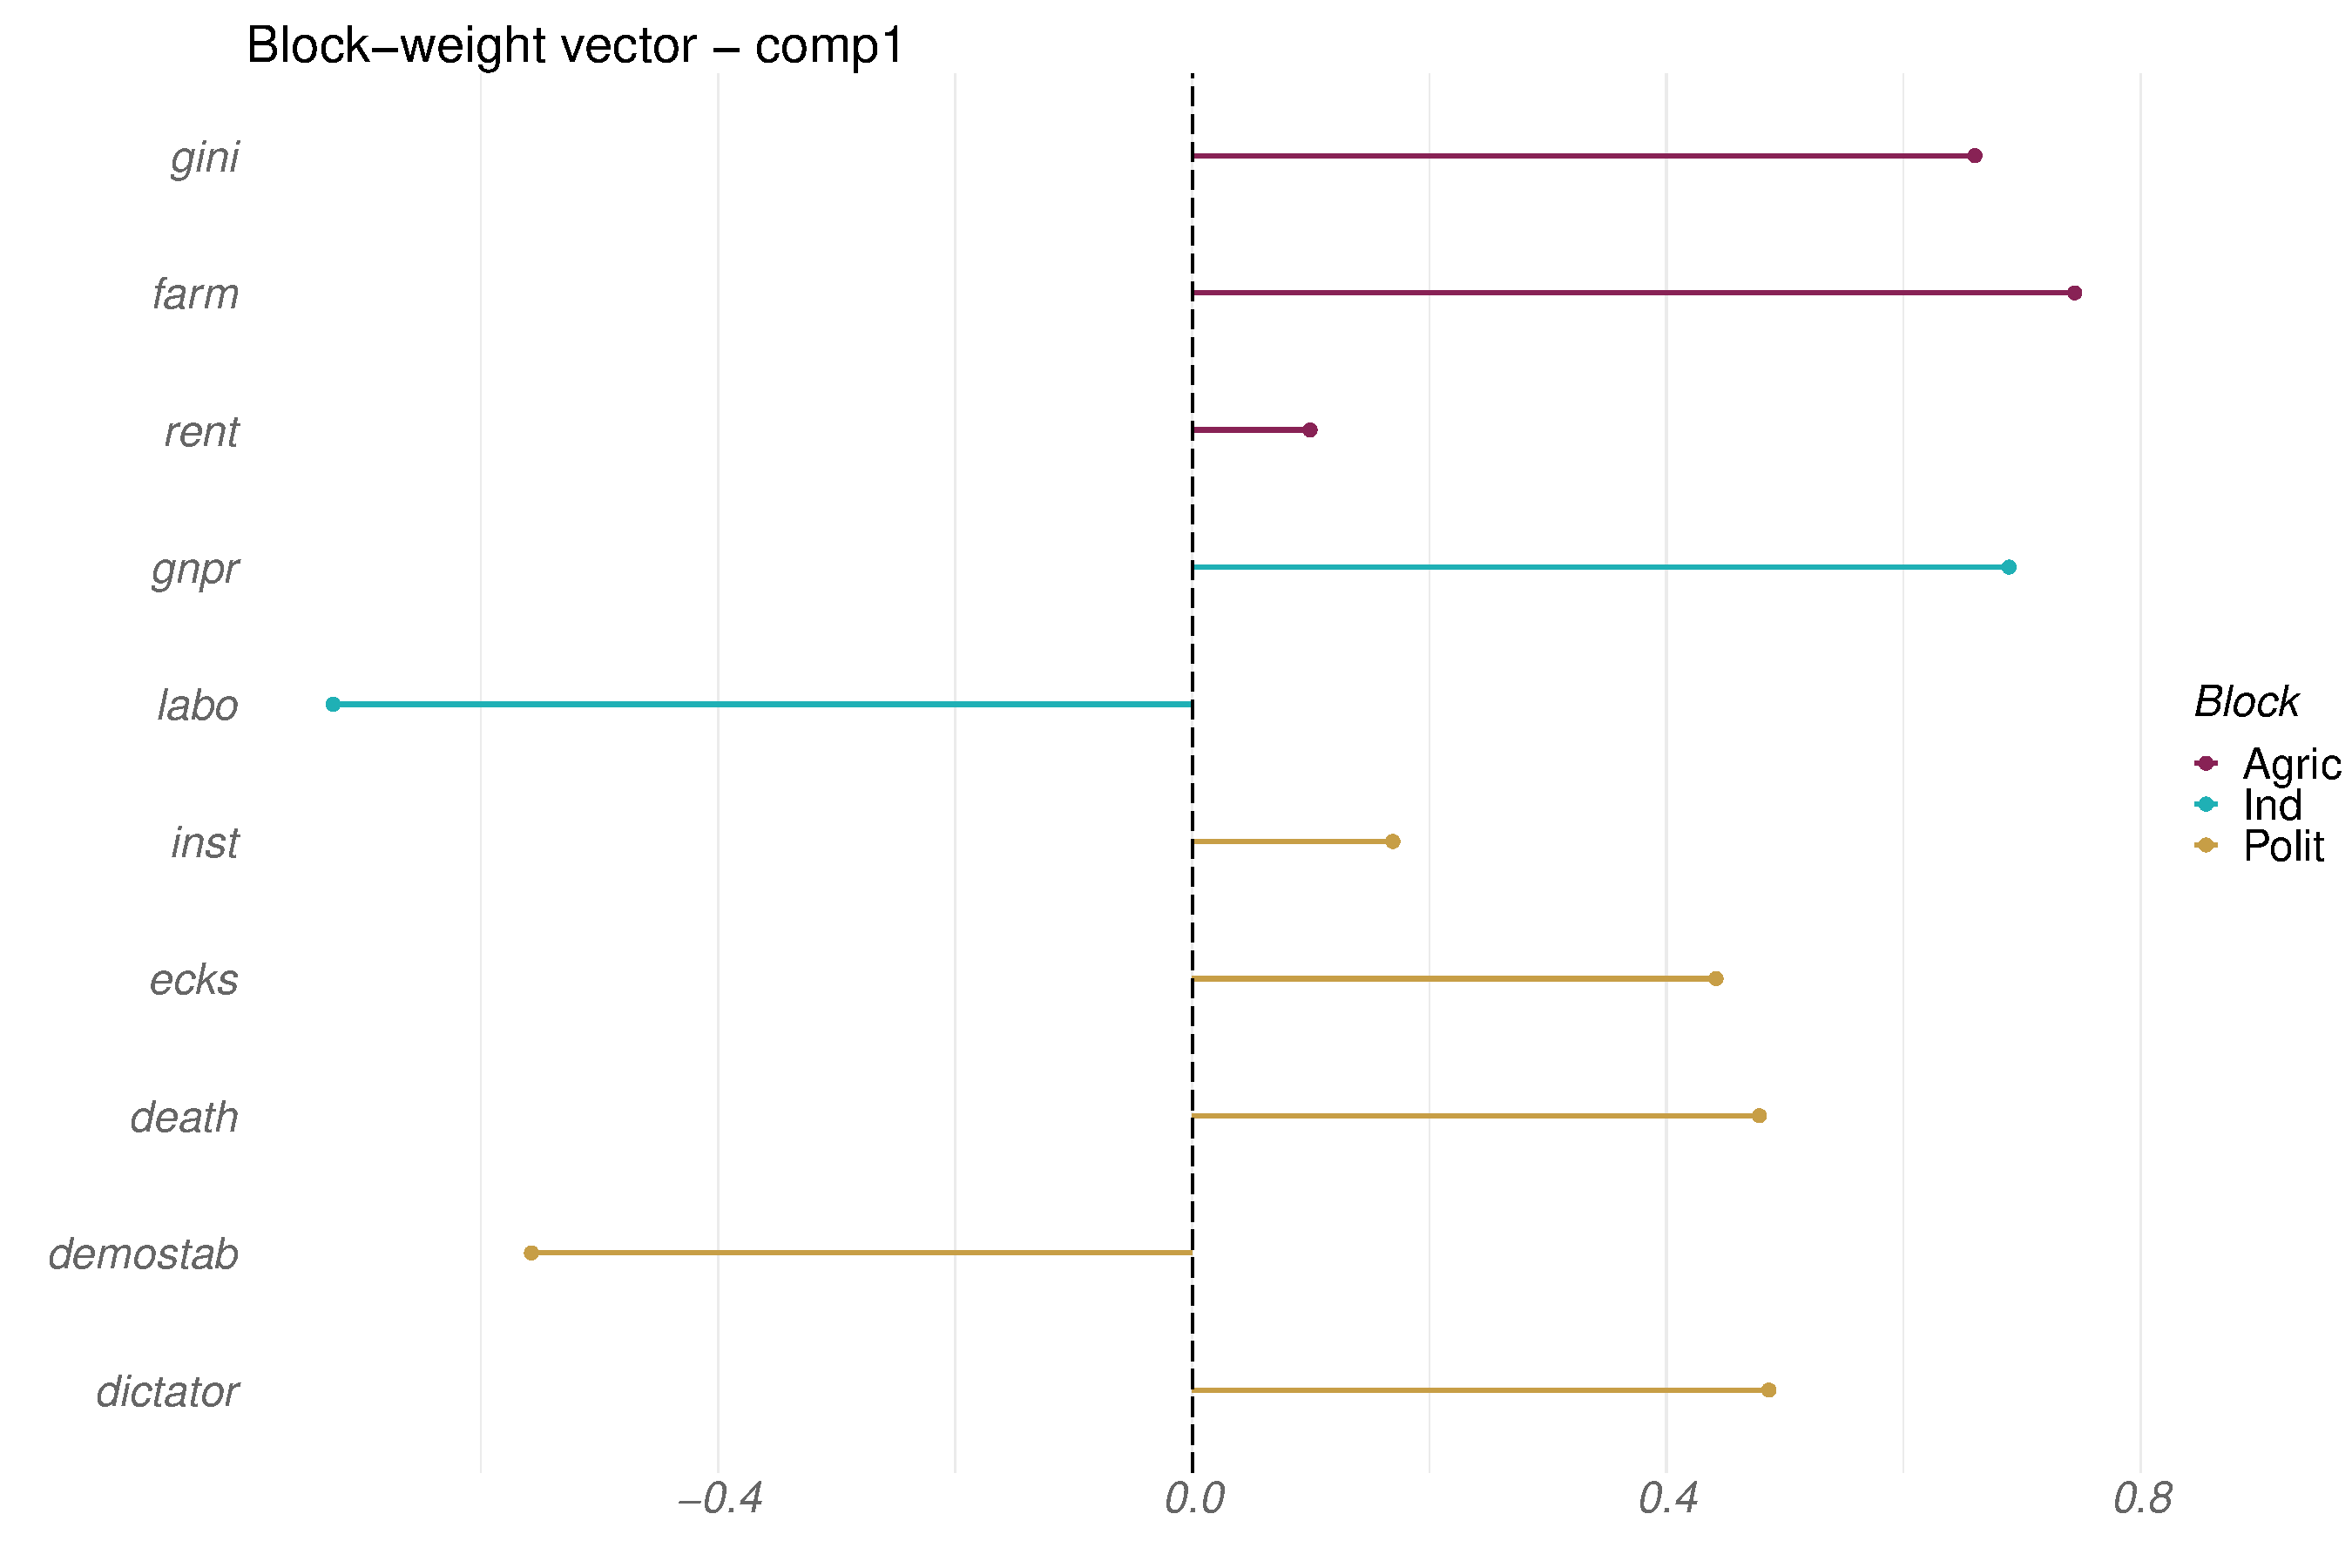
\includegraphics{figures/unnamed-chunk-8-1} 

}

\caption[Block-weight vectors of a fitted RGCCA model]{Block-weight vectors of a fitted RGCCA model.}\label{fig:unnamed-chunk-8}
\end{figure}
\end{CodeChunk}

\normalsize

As a component-based method, the RGCCA package provides block components
as output of the \(\small{\texttt{rgcca()}}\) function in
\(\small{\texttt{fit\$Y}}\) and graphical representations, including
factor plot (\(\small{\texttt{type = "sample"}}\)), correlation circle
(\(\small{\texttt{type = "cor\_circle"}}\)) or biplot
(\(\small{\texttt{type = "biplot"}}\)). This graphical display allows
visualizing the sources of variability within blocks, the relationships
between variables within and between blocks, and the amount of
correlation between blocks. The graphical display of the countries
obtained by crossing \(\mathbf X_1 \mathbf a_1\) = Agricultural
Inequality and \(\mathbf X_2 \mathbf a_2\) = Industrial Development and
marked with their political regime in 1960 is shown below.

\footnotesize

\begin{CodeChunk}
\begin{CodeInput}
R> plot(fit, type = "sample",
+      block = 1:2, comp = 1,
+      resp = lab, repel = TRUE, cex = 2)
\end{CodeInput}
\begin{figure}[H]

{\centering 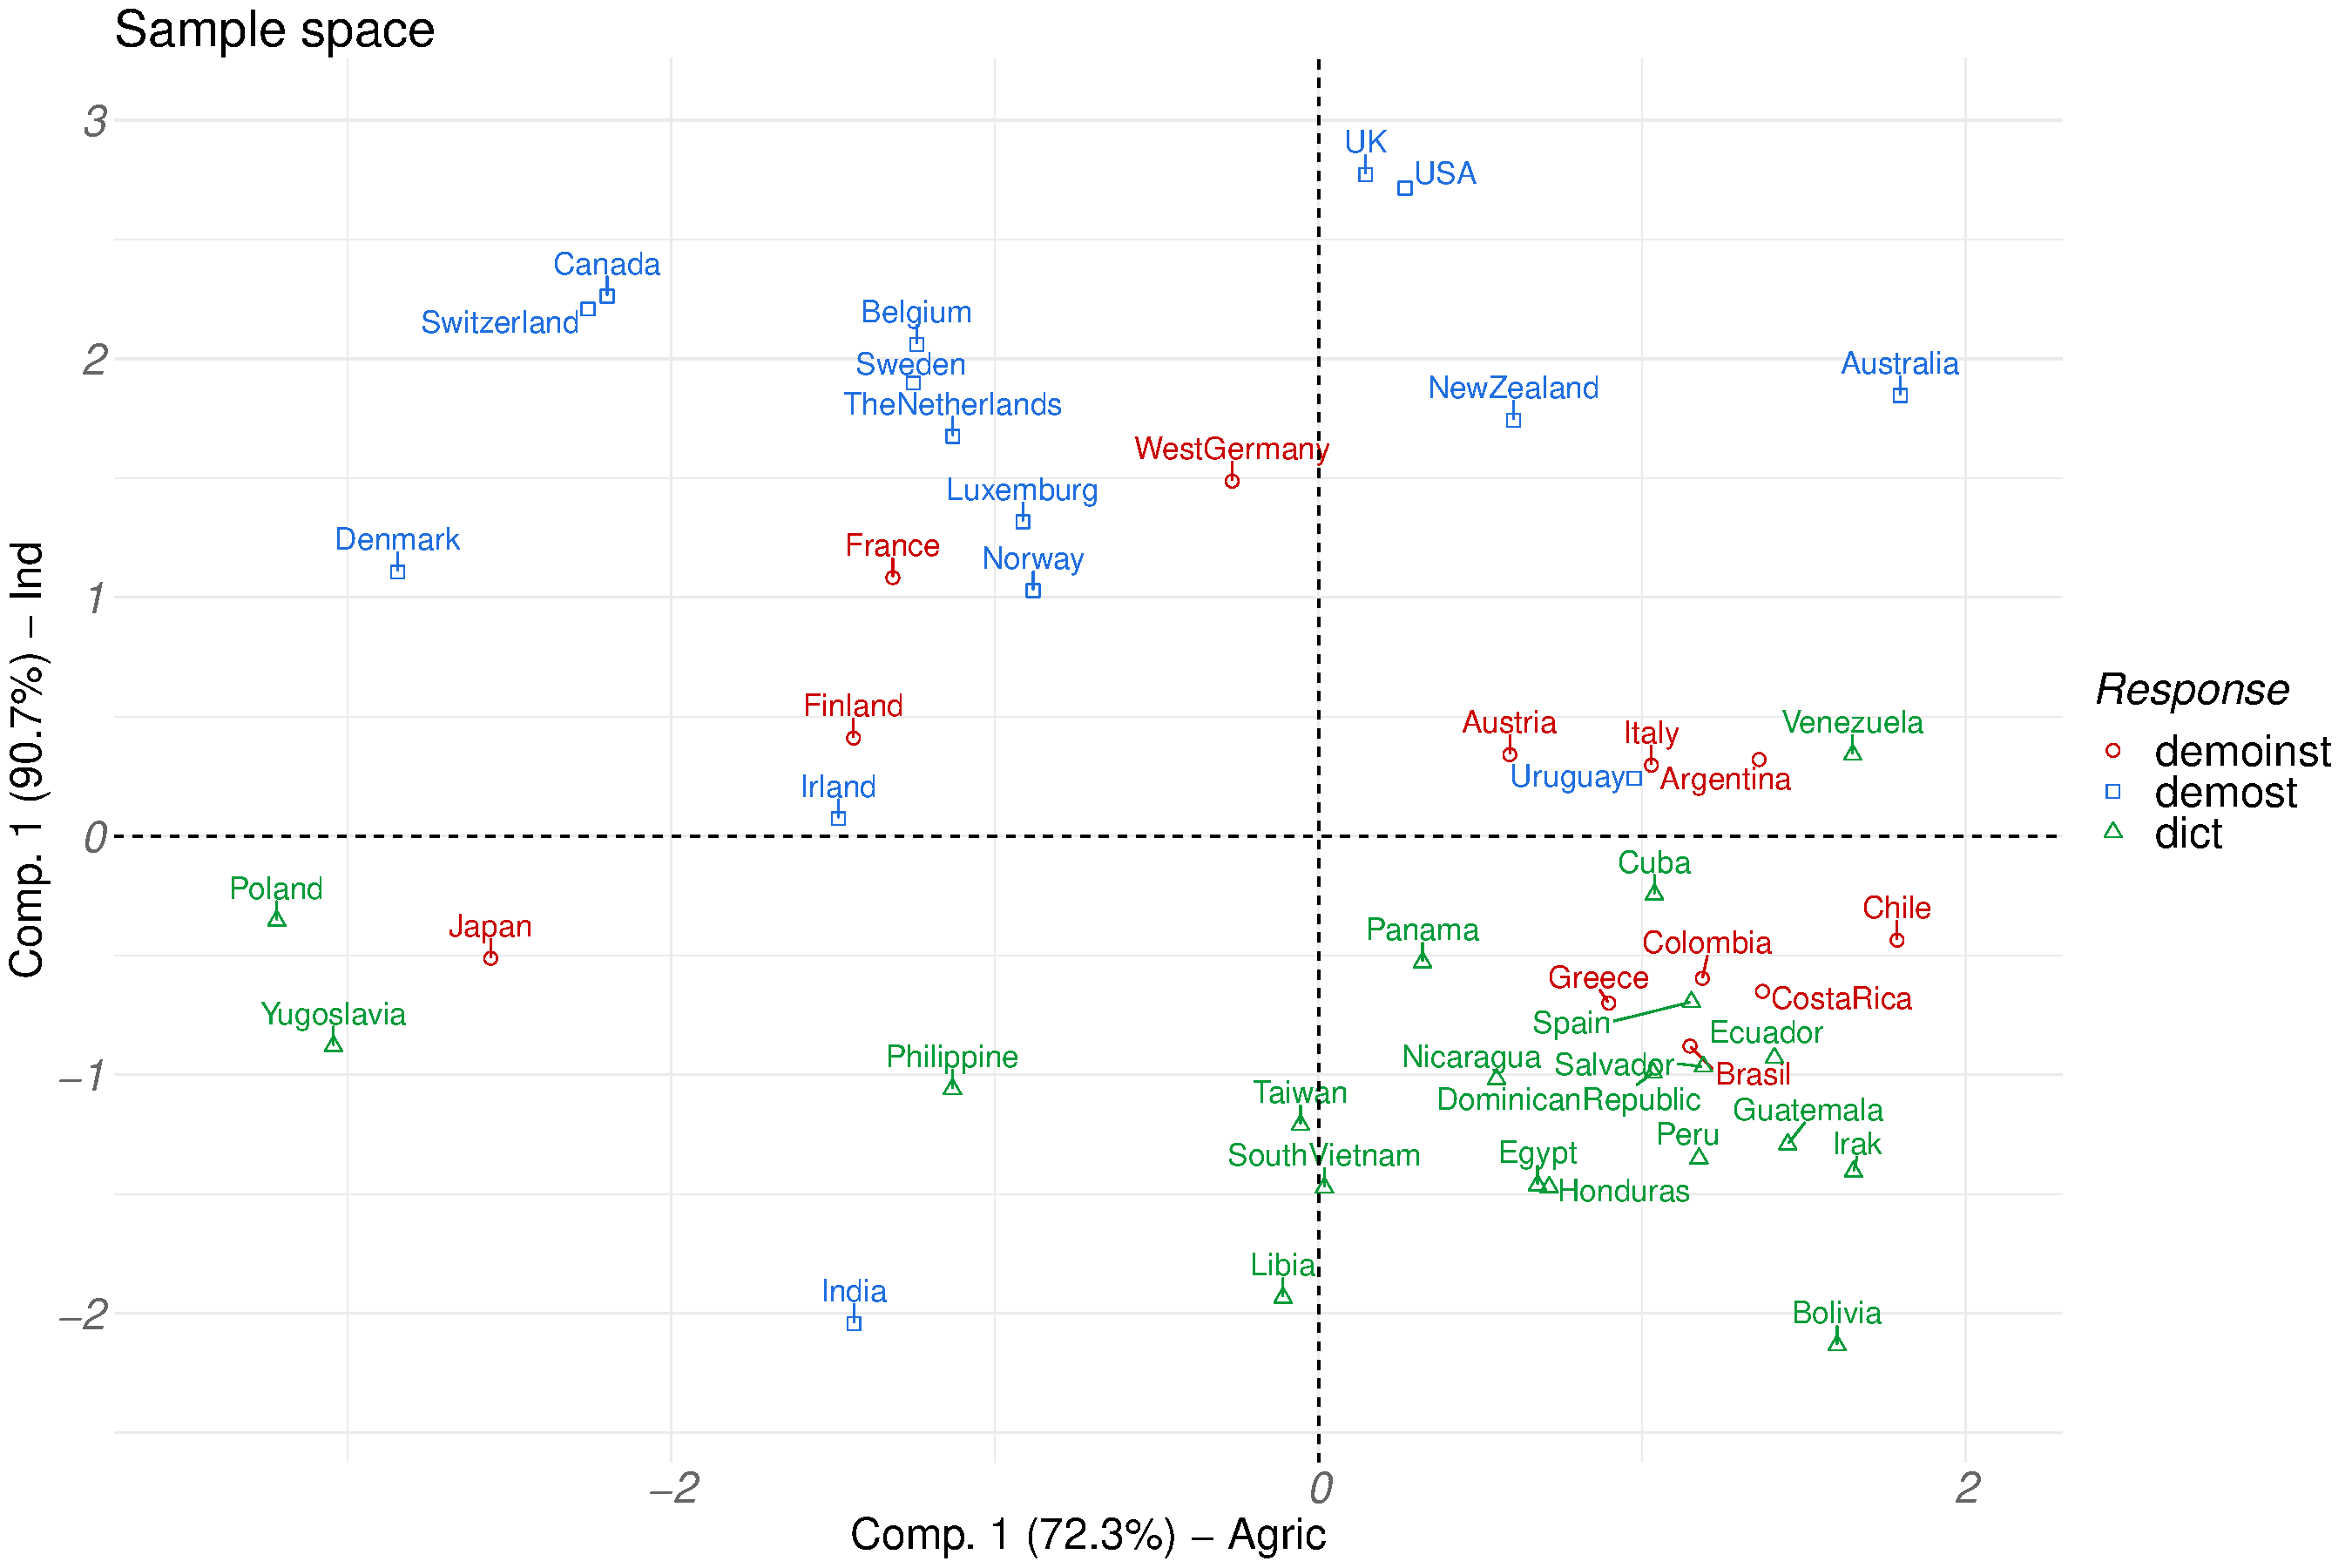
\includegraphics{figures/unnamed-chunk-9-1} 

}

\caption{\label{fig:sample}Graphical display of the countries by drawing the block component of the first block against the block component of the second block, colored according to their political regime.}\label{fig:unnamed-chunk-9}
\end{figure}
\end{CodeChunk}

\normalsize

Countries aggregate together when they share similarities. It may be
noted that the lower right quadrant concentrates on dictatorships. It is
difficult for a country to escape dictatorship when its industrial
development is below average, and its agricultural inequality is above
average. It is worth pointing out that some unstable democracies located
in this quadrant (or close to it) became dictatorships for a period of
time after 1960: Greece (1967-1974), Brazil (1964-1985), Chili
(1973-1990), and Argentina (1966-1973).

The AVEs of the different blocks are reported in the axes of Figure
\ref{fig:sample}. All AVEs (defined in \ref{AVE_X}-\ref{AVE_inner}) are
available as output of the \(\small{\texttt{rgcca()}}\) function in
\(\small{\texttt{fit\$AVE}}\). These indicators of model quality can
also be visualized using the generic \(\small{\texttt{plot()}}\)
function.

\footnotesize

\begin{CodeChunk}
\begin{CodeInput}
R> plot(fit, type = "ave", cex = 2)
\end{CodeInput}
\begin{figure}[H]

{\centering 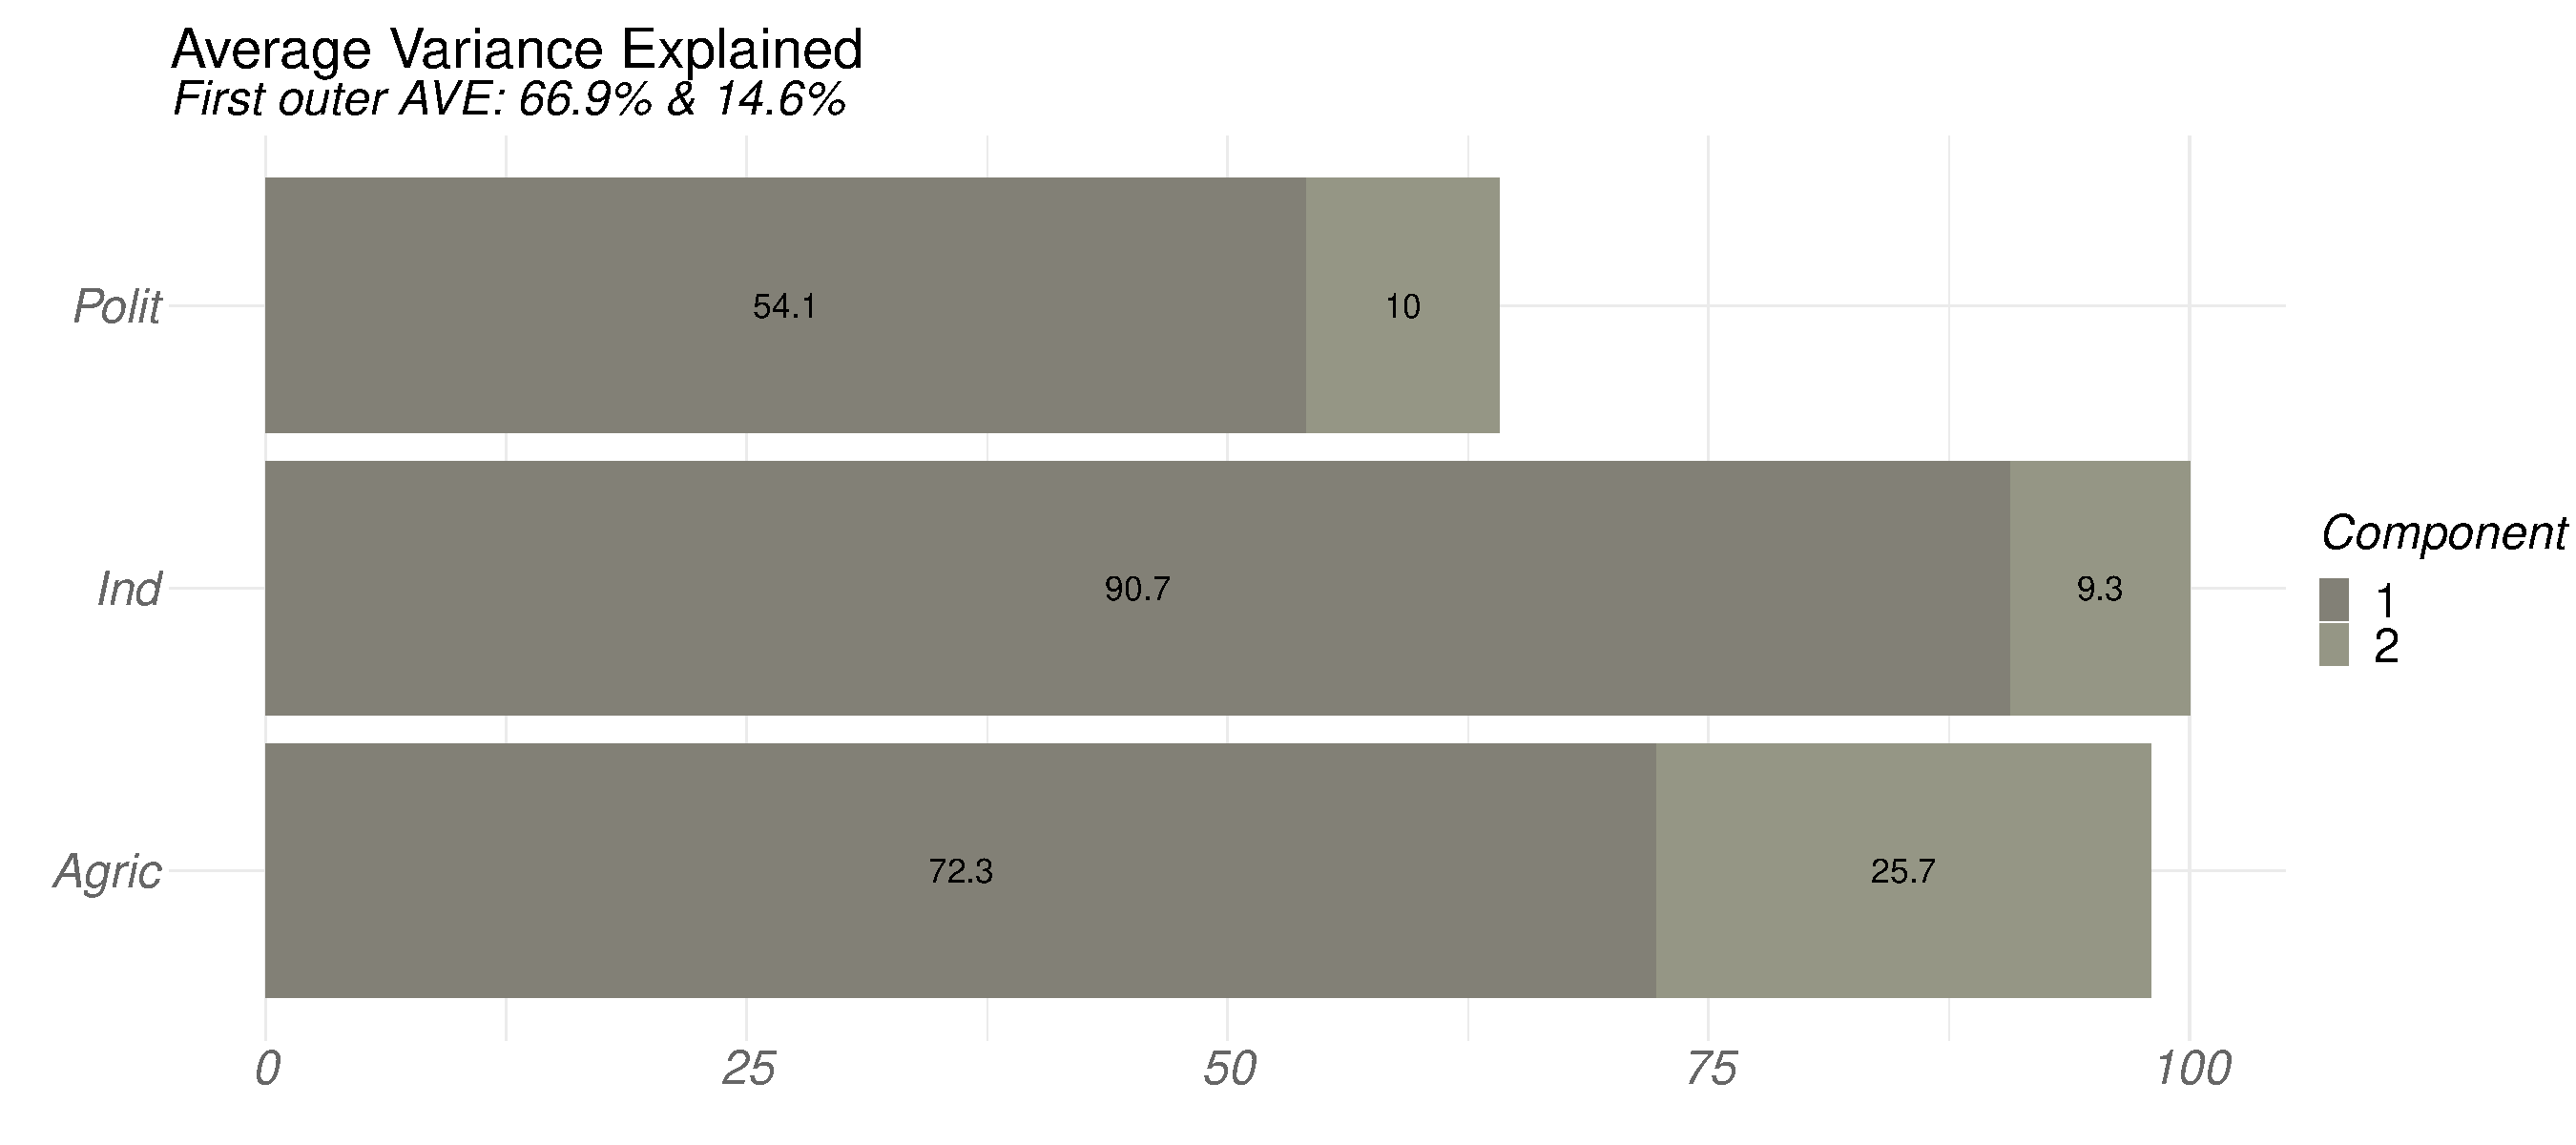
\includegraphics{figures/unnamed-chunk-10-1} 

}

\caption[Average Variance Explained of the different blocks]{Average Variance Explained of the different blocks.}\label{fig:unnamed-chunk-10}
\end{figure}
\end{CodeChunk}

\normalsize

The strength of the relations between each block component and each
variable can be visualized using correlation circles or biplot
representations.

\footnotesize

\begin{CodeChunk}
\begin{CodeInput}
R> plot(fit, type = "cor_circle", block = 1, comp = 1:2, 
+      display_blocks = 1:3, cex = 2)
\end{CodeInput}
\begin{figure}[H]

{\centering 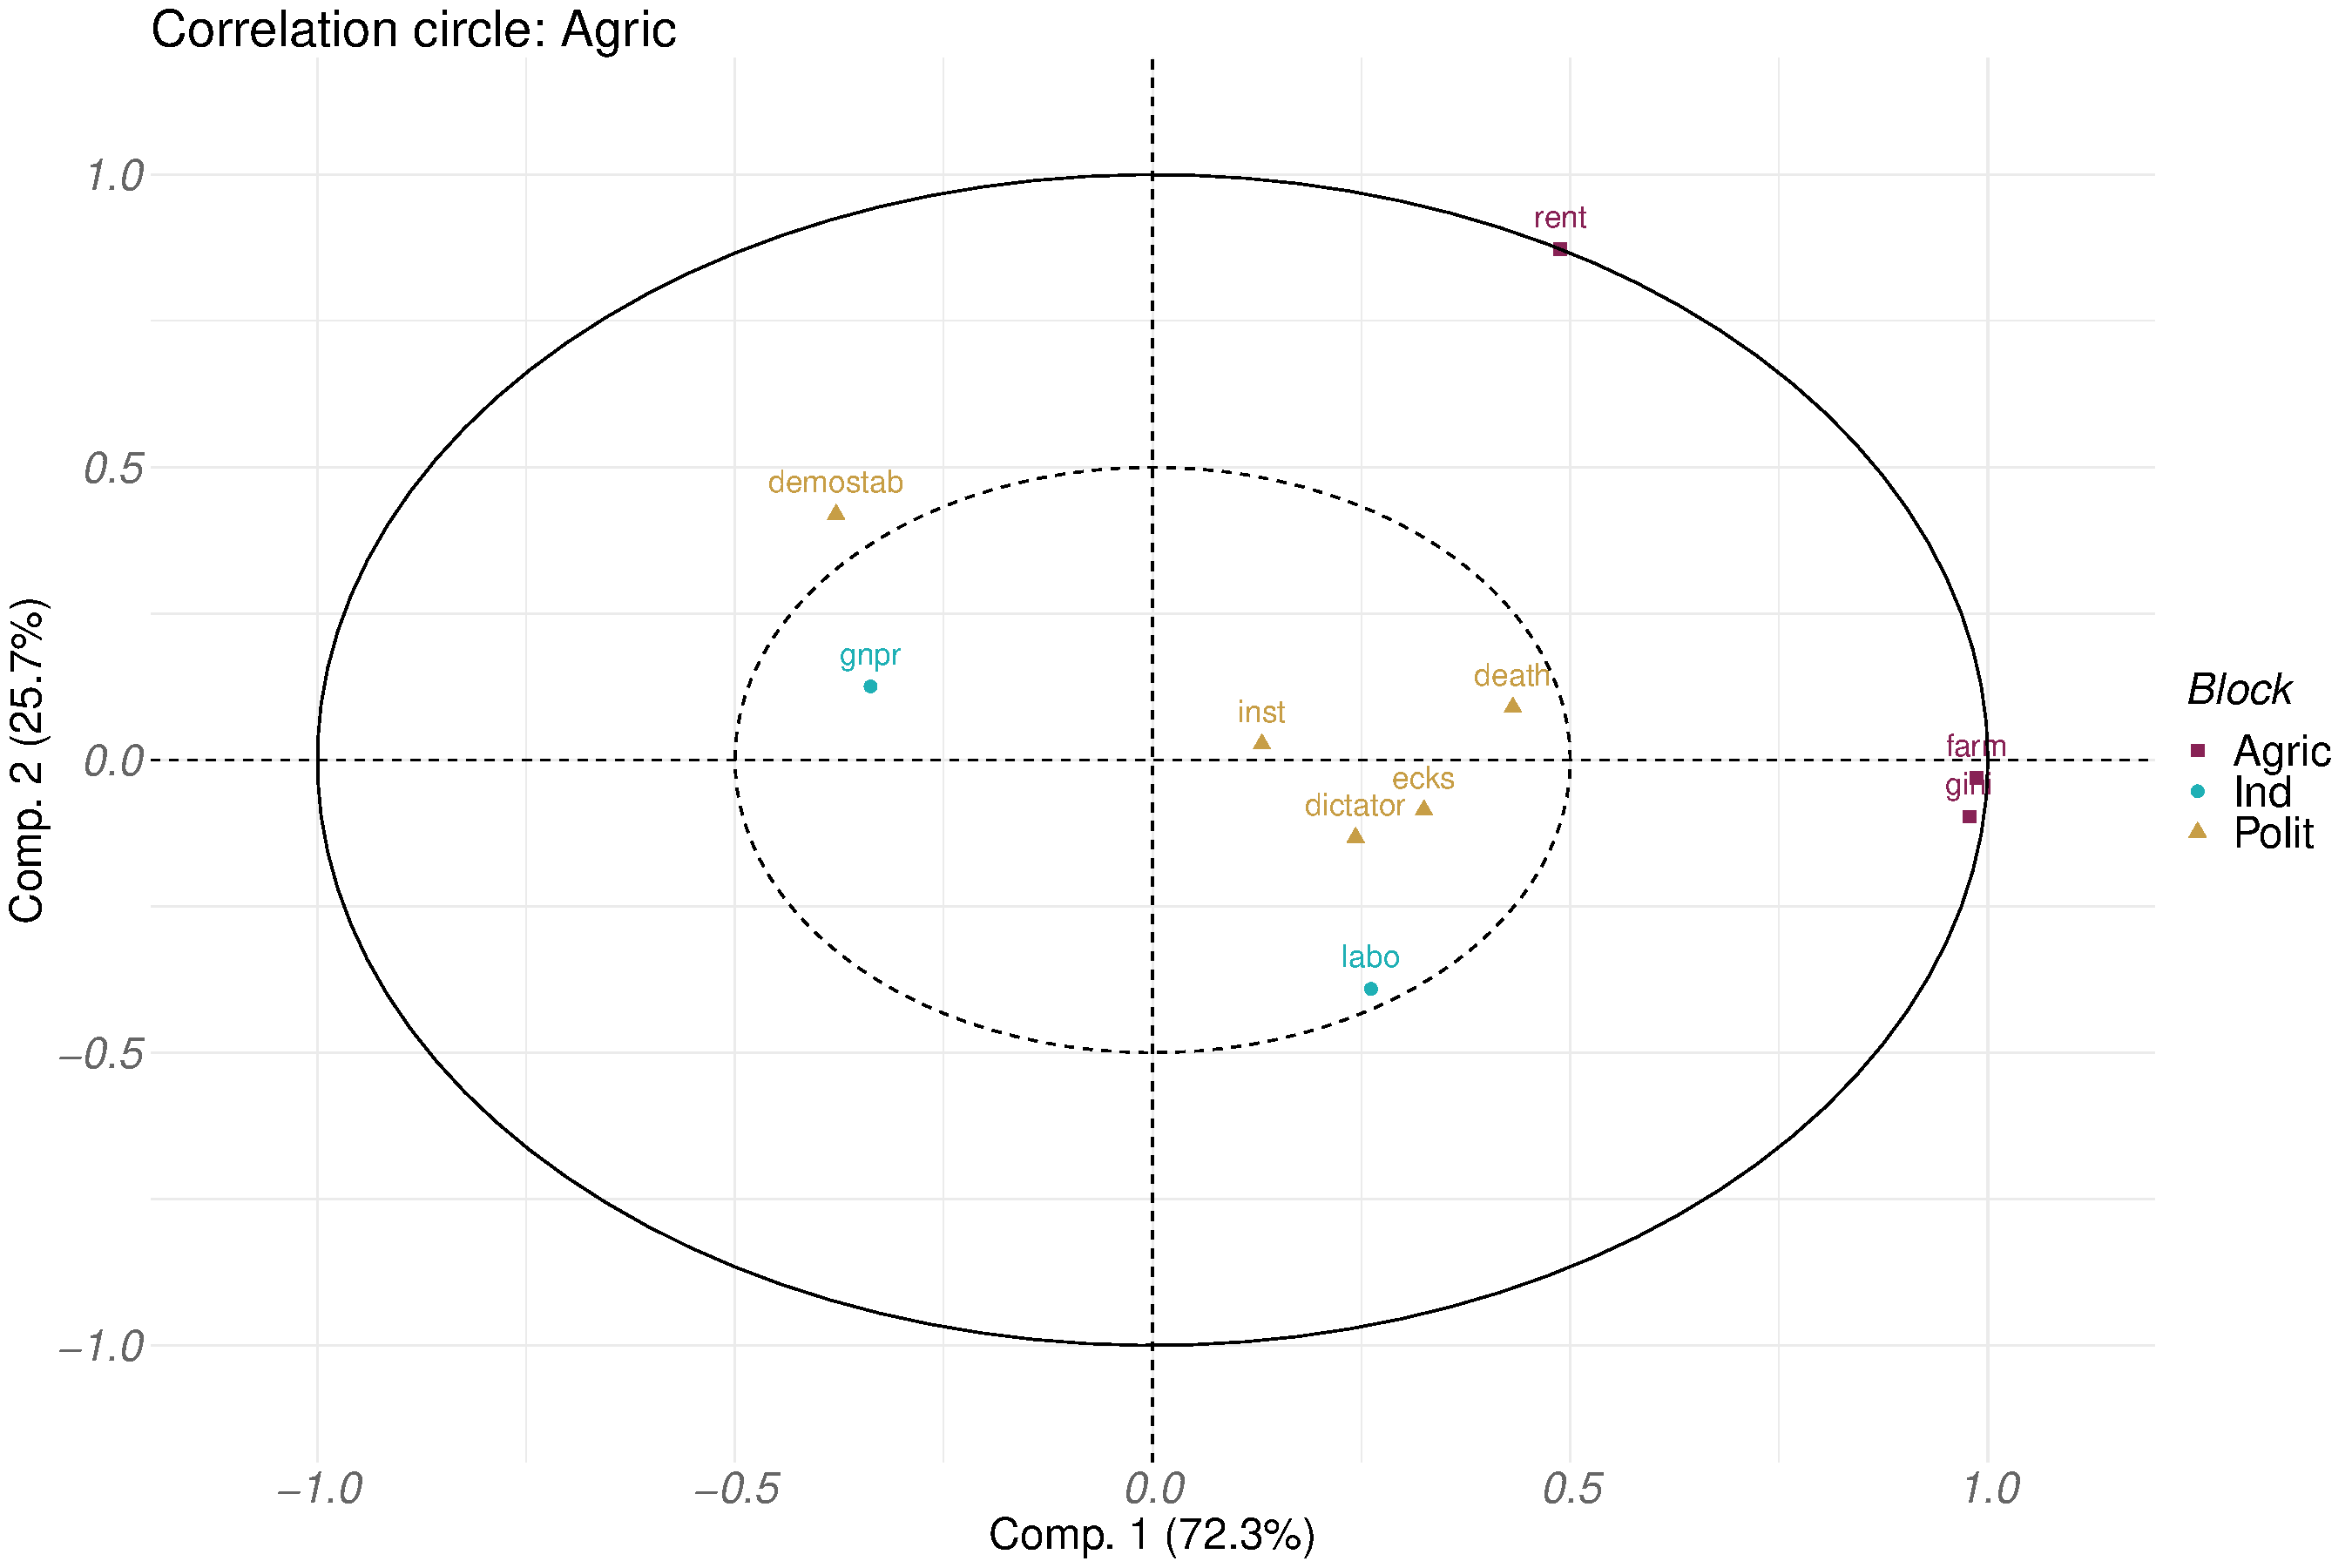
\includegraphics{figures/unnamed-chunk-11-1} 

}

\caption[Correlation circle associated with the first two components of the Agriculture block]{Correlation circle associated with the first two components of the Agriculture block.}\label{fig:unnamed-chunk-11}
\end{figure}
\end{CodeChunk}

\normalsize

By default, all the variables are displayed on the correlation circle.
However, it is possible to choose the block(s) to display
(\(\small{\texttt{display\_blocks}}\)) in the correlation\_circle.

\footnotesize

\begin{CodeChunk}
\begin{CodeInput}
R> plot(fit, type = "biplot", block = 1, 
+      comp = 1:2, repel = TRUE, 
+      resp = lab, cex = 2,
+      show_arrow = TRUE)
\end{CodeInput}
\begin{figure}[H]

{\centering 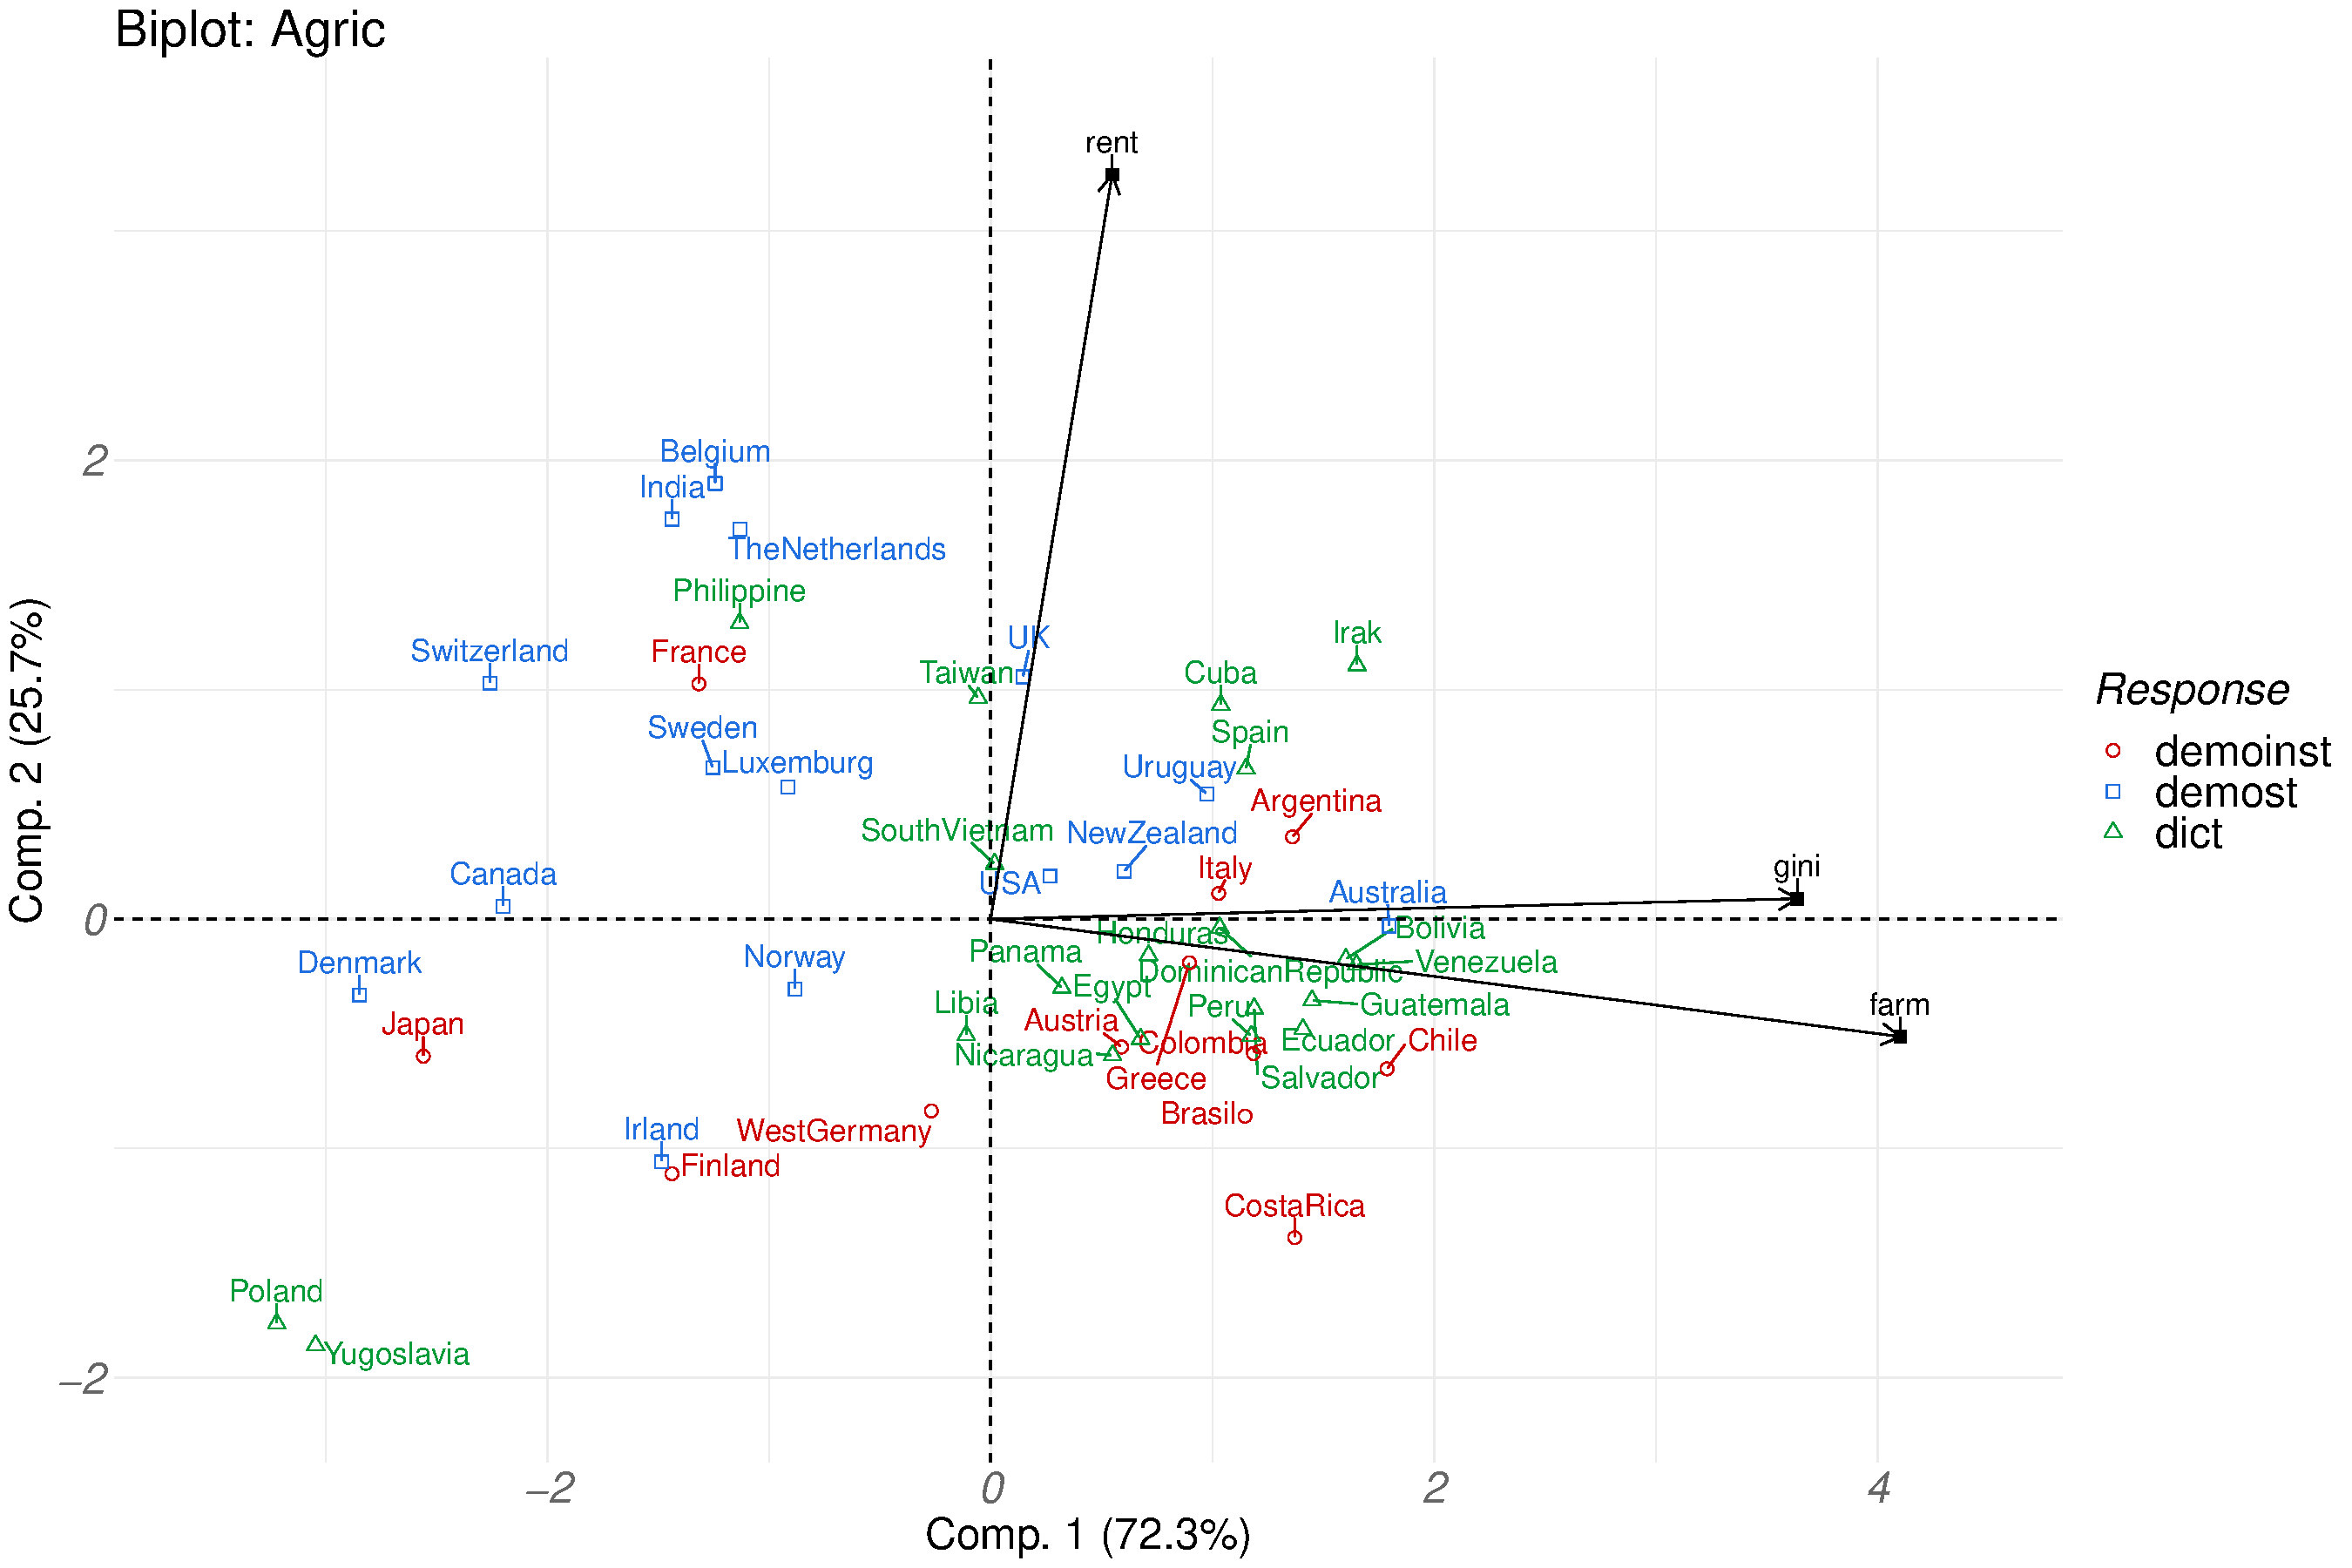
\includegraphics{figures/unnamed-chunk-12-1} 

}

\caption[Biplot associated with the first two components ofthe Agriculture block]{Biplot associated with the first two components ofthe Agriculture block.}\label{fig:unnamed-chunk-12}
\end{figure}
\end{CodeChunk}

\normalsize

As we will see in the next section, when the superblock option is
considered (\(\small{\texttt{superblock = TRUE}}\) or
\(\small{\texttt{method}}\) set to a method that induces the use of
superblock), global components can be derived. The space spanned by the
global components can be viewed as a consensus space that integrates all
the modalities and facilitates the visualization of the results and
their interpretation.

\textbf{Assessment of the reliability of parameter estimates.} It is
possible to use a bootstrap resampling method to assess the reliability
of parameter estimates (block-weight/loading vectors) obtained using
RGCCA. \(\small{\texttt{B = n\_boot}}\) bootstrap samples of the same
size as the original data are repeatedly sampled with replacement from
the original data. RGCCA is then applied to each bootstrap sample to
obtain the RGCCA estimates. We calculate the standard deviation of the
estimates across the bootstrap samples, from which we derive bootstrap
confidence intervals, t-ratio (defined as the ratio of the parameter
estimate to its bootstrap estimate of the standard deviation), and
p-value (the p-value is computed by assuming that the ratio of the
parameter estimate to its standard deviation follows the standardized
normal distribution), to indicate how reliably parameters were
estimated. Since several p-values are constructed simultaneously, FDR
correction can be applied to control the False Discovery Rate. This
function is available using the \(\small{\texttt{rgcca\_bootstrap()}}\)
function of the RGCCA package.

\footnotesize

\begin{CodeChunk}
\begin{CodeInput}
R> boot_out <- rgcca_bootstrap(fit, n_boot = 500, n_cores = 1)
\end{CodeInput}
\end{CodeChunk}

\normalsize

The bootstrap results are detailed using the
\(\small{\texttt{print()}}\) function,

\footnotesize

\begin{CodeChunk}
\begin{CodeInput}
R> print(boot_out, block = 1:3, ncomp = 1)
\end{CodeInput}
\begin{CodeOutput}
Call: method='rgcca', superblock=FALSE, scale=TRUE, scale_block=FALSE, init='svd',
bias=TRUE, tol=1e-08, NA_method='na.ignore', ncomp=c(2,2,2), response=NULL,
comp_orth=TRUE 
There are J = 3 blocks.
The design matrix is:
      Agric Ind Polit
Agric     0   0     1
Ind       0   0     1
Polit     1   1     0

The factorial scheme is used.

Extracted statistics from 500 bootstrap samples.
Block-weight vectors for component 1: 
         estimate    mean     sd lower_bound upper_bound bootstrap_ratio  pval
gini       0.6602  0.6369 0.0703      0.4947       0.728           9.389 0.000
farm       0.7445  0.7306 0.0481      0.6452       0.832          15.476 0.000
rent       0.0994  0.0741 0.2191     -0.4255       0.416           0.454 0.484
gnpr       0.6891  0.6883 0.0313      0.6222       0.738          22.020 0.000
labo      -0.7247 -0.7241 0.0288     -0.7829      -0.675         -25.131 0.000
inst       0.1692  0.1663 0.1056     -0.0613       0.341           1.602 0.073
ecks       0.4418  0.4362 0.0596      0.3171       0.551           7.411 0.000
death      0.4784  0.4714 0.0509      0.3645       0.567           9.395 0.000
demostab  -0.5574 -0.5520 0.0505     -0.6553      -0.452         -11.037 0.000
dictator   0.4864  0.4827 0.0488      0.3808       0.575           9.973 0.000
         adjust.pval
gini           0.000
farm           0.000
rent           0.569
gnpr           0.000
labo           0.000
inst           0.104
ecks           0.000
death          0.000
demostab       0.000
dictator       0.000
\end{CodeOutput}
\end{CodeChunk}

\normalsize

and displayed using the \(\small{\texttt{plot()}}\) function.

\footnotesize

\begin{CodeChunk}
\begin{CodeInput}
R> plot(boot_out, type = "weight", 
+      block = 1:3, comp = 1, 
+      display_order = FALSE, cex = 2,
+      show_stars = TRUE)
\end{CodeInput}
\begin{figure}[H]

{\centering 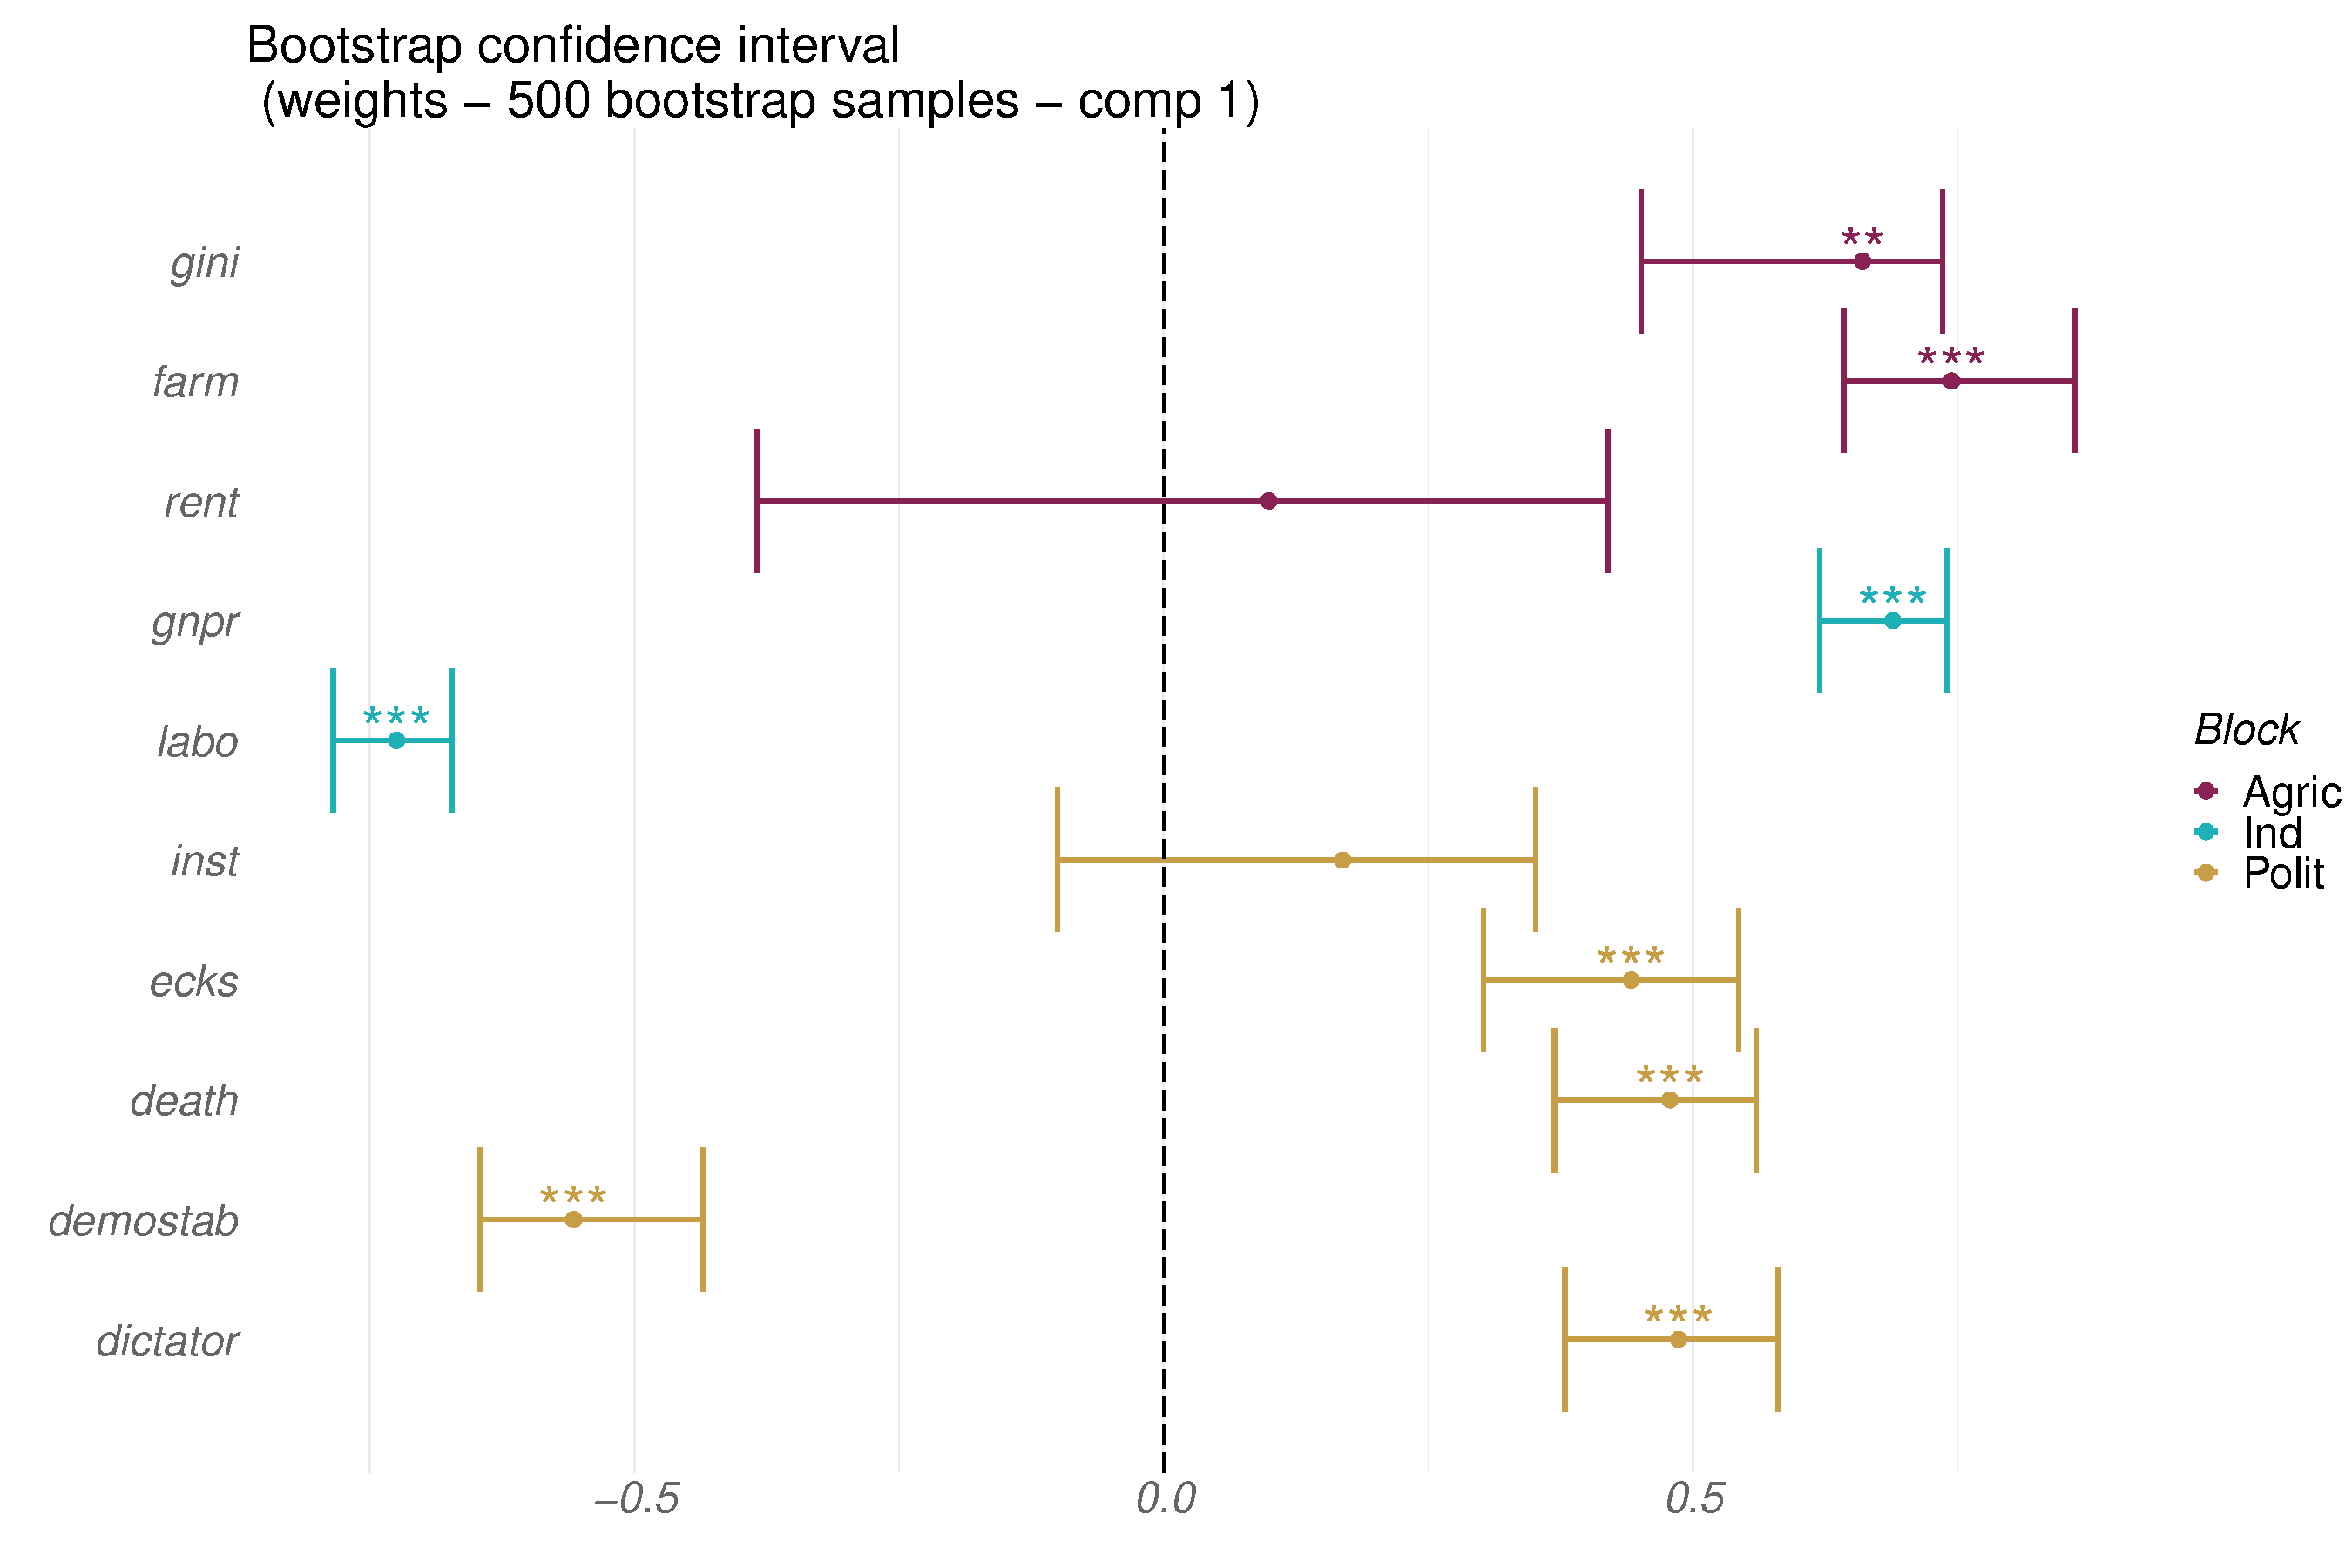
\includegraphics{figures/unnamed-chunk-15-1} 

}

\caption[Bootstrap confidence intervals for the block-weight vectors]{Bootstrap confidence intervals for the block-weight vectors.}\label{fig:unnamed-chunk-15}
\end{figure}
\end{CodeChunk}

\normalsize

Each weight is shown along with its associated bootstrap confidence
interval and stars (\(\small{\texttt{show\_stars = TRUE}}\)) reflecting
the p-value of assigning a strictly positive or negative weight to this
variable.

\hypertarget{rgcca-with-superblock}{%
\subsection{RGCCA with superblock}\label{rgcca-with-superblock}}

In this section, we consider Multiple Co-Inertia Analysis
\citep{Chessel1996} \citep[MCOA, also called MCIA in][]{Cantini2021}
with \(2\) components per block.

See \(\small{\texttt{available\_methods()}}\) for a list of
pre-specified multiblock component methods.

\footnotesize

\begin{CodeChunk}
\begin{CodeInput}
R> fit.mcoa <- rgcca(blocks = A, method = "mcoa", ncomp = 2)
\end{CodeInput}
\end{CodeChunk}

\normalsize

Interestingly, the \(\small{\texttt{print()}}\) function reports the
arguments implicitly specified to perform MCOA.

\footnotesize

\begin{CodeChunk}
\begin{CodeInput}
R> print(fit.mcoa)
\end{CodeInput}
\begin{CodeOutput}
Call: method='mcoa', superblock=TRUE, scale=TRUE, scale_block='inertia', init='svd',
bias=TRUE, tol=1e-08, NA_method='na.ignore', ncomp=c(2,2,2,2), response=NULL,
comp_orth=FALSE 
There are J = 4 blocks.
The design matrix is:
           Agric Ind Polit superblock
Agric          0   0     0          1
Ind            0   0     0          1
Polit          0   0     0          1
superblock     1   1     1          0

The factorial scheme is used.
Sum_{j,k} c_jk g(cov(X_j a_j, X_k a_k) = 3.578 

The regularization parameter used for Agric is: 1
The regularization parameter used for Ind is: 1
The regularization parameter used for Polit is: 1
The regularization parameter used for superblock is: 0
\end{CodeOutput}
\end{CodeChunk}

\normalsize

It is possible to display specific output as previously using the
generic \(\small{\texttt{plot()}}\) function by specifying the argument
\(\small{\texttt{type}}\) accordingly. MCOA enables individuals to be
represented in the space spanned by the first global components. The
biplot representation associated with this consensus space is given
below.

\footnotesize

\begin{CodeChunk}
\begin{CodeInput}
R> plot(fit.mcoa, type = "biplot", 
+      block = 4, comp = 1:2, 
+      response = lab, 
+      repel = TRUE, cex = 2)
\end{CodeInput}
\begin{figure}[H]

{\centering 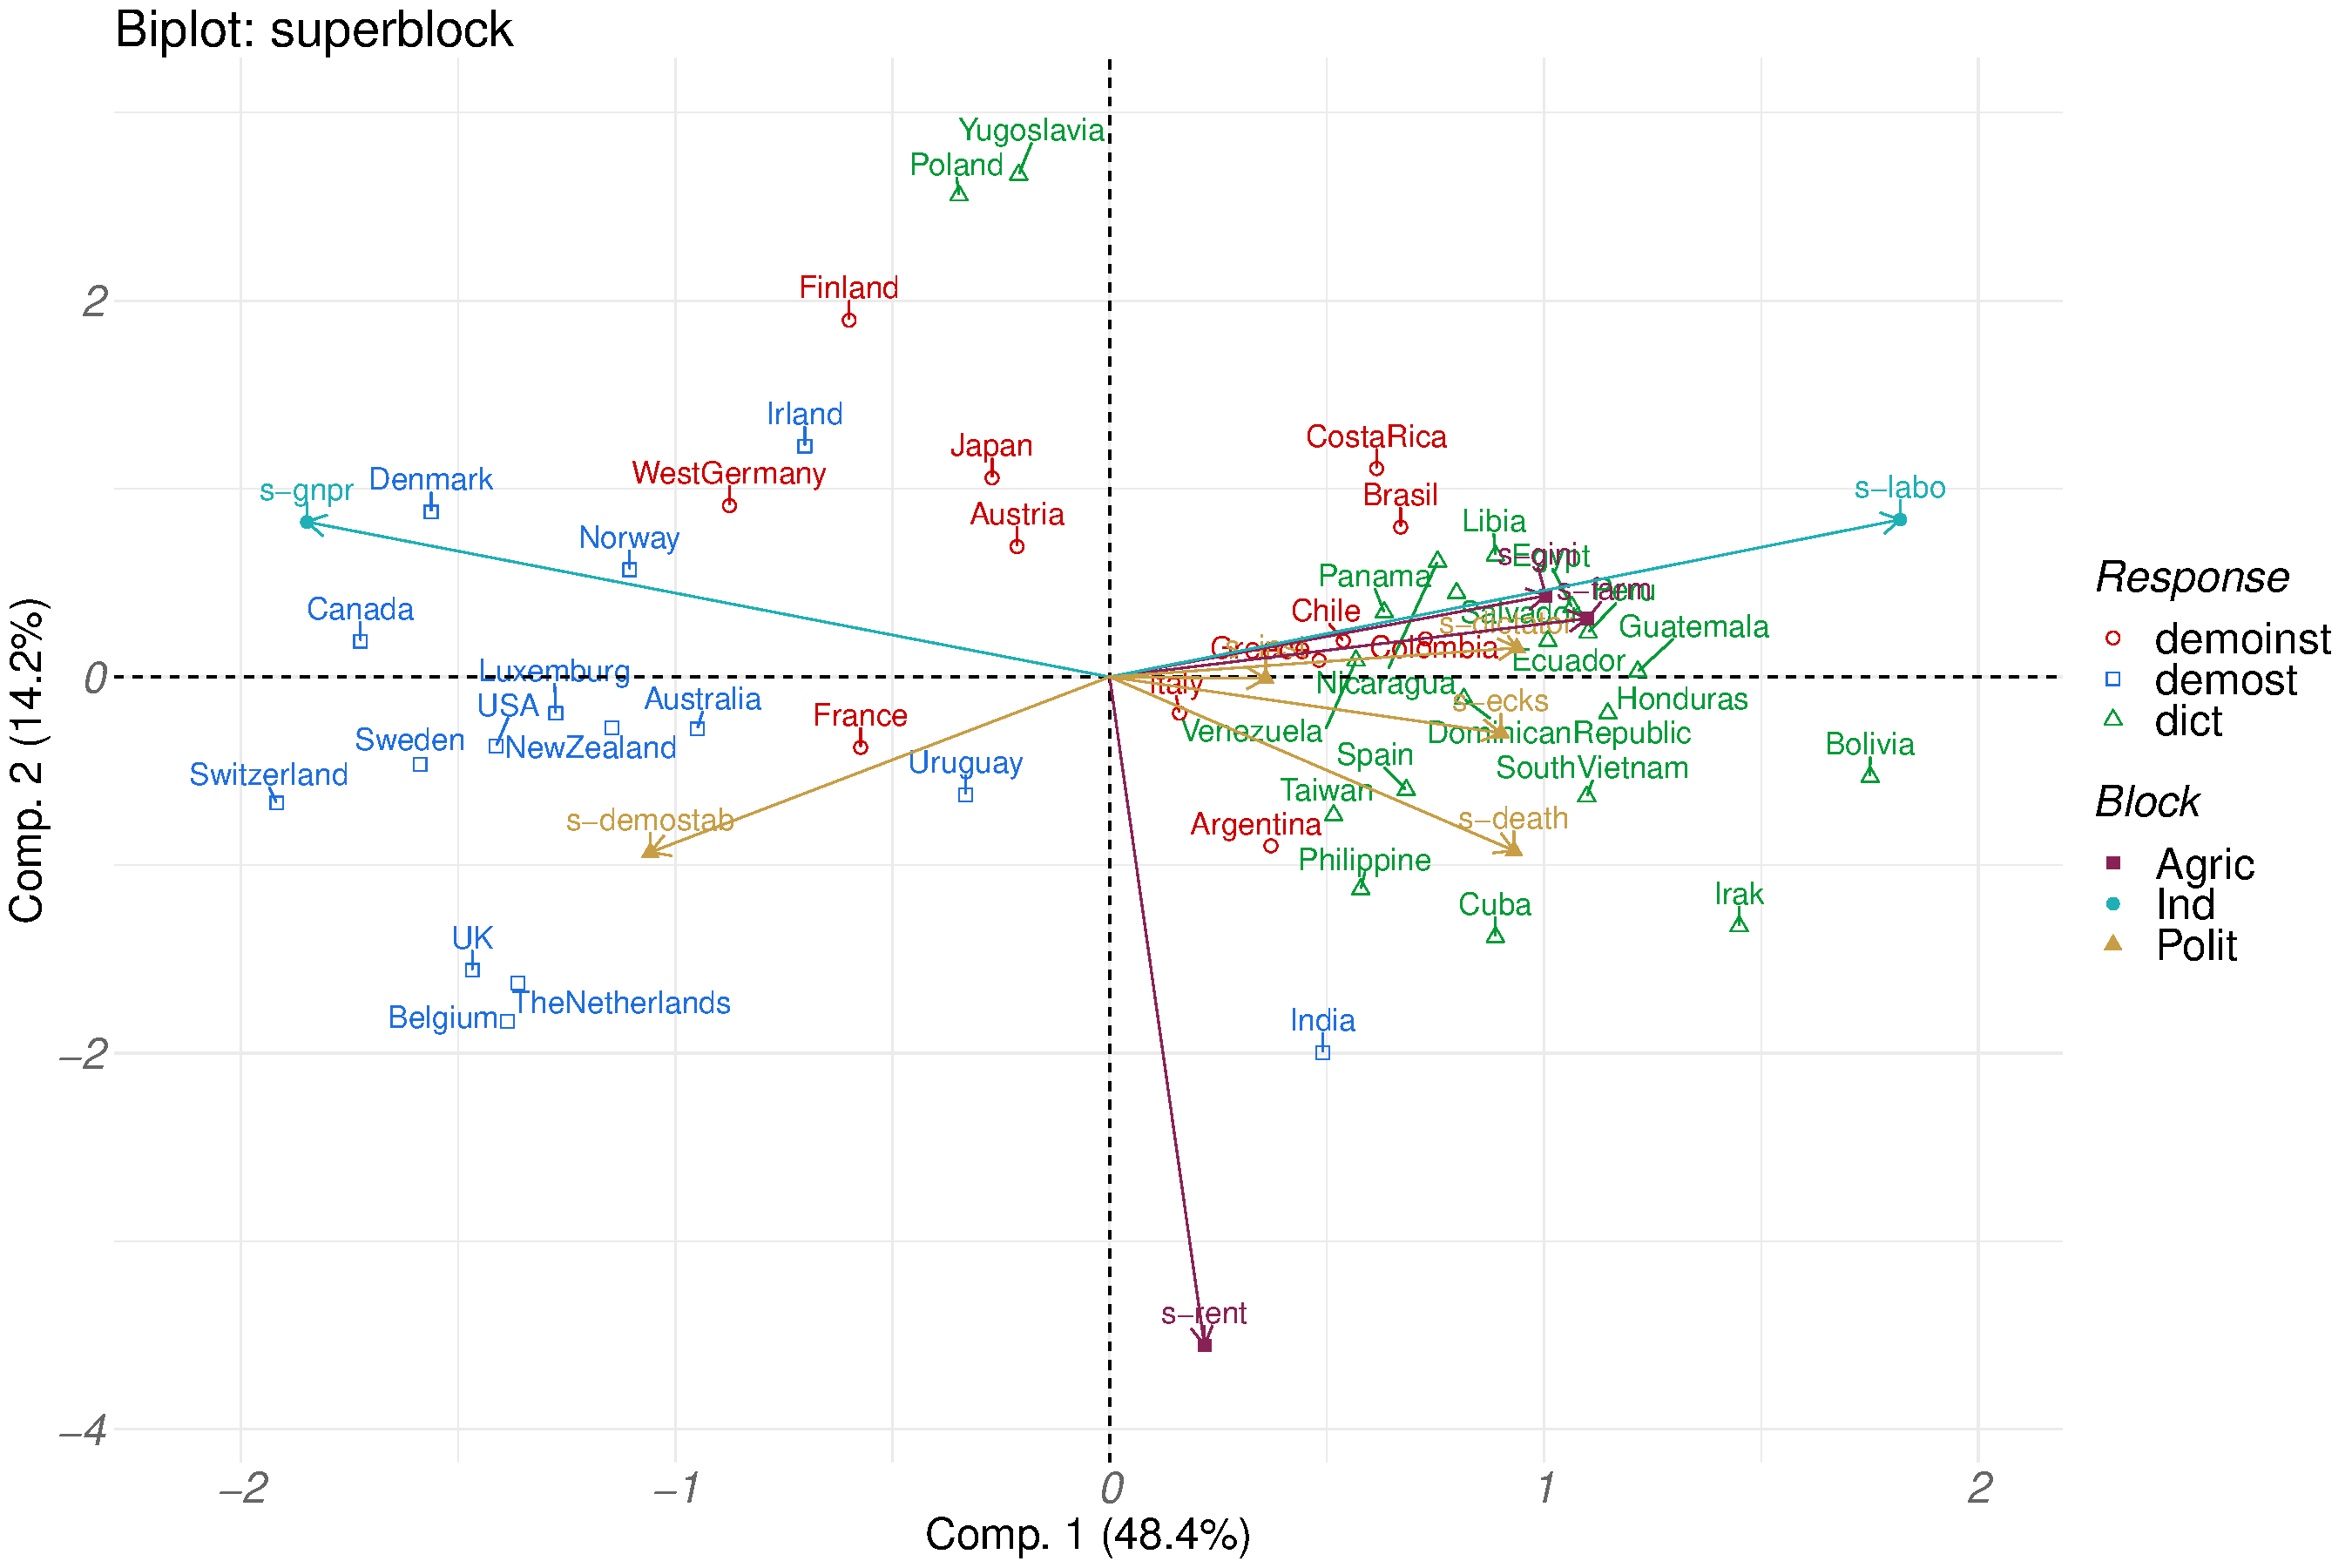
\includegraphics{figures/unnamed-chunk-18-1} 

}

\caption[Biplot of the countries obtained by crossing the two first components of the superblock]{Biplot of the countries obtained by crossing the two first components of the superblock. Individuals are colored according to their political regime and variables according to their block membership.}\label{fig:unnamed-chunk-18}
\end{figure}
\end{CodeChunk}

\normalsize

As previously, this model can be easily bootstrapped using the
\(\small{\texttt{rgcca\_bootstrap()}}\) function, and the bootstrap
confidence intervals are still available using the
\(\small{\texttt{print()}}\) and \(\small{\texttt{plot()}}\) functions.

\hypertarget{choice-of-the-shrinkage-parameters}{%
\subsection{Choice of the shrinkage
parameters}\label{choice-of-the-shrinkage-parameters}}

Three fully automatic strategies are proposed to select the optimal
shrinkage parameters:

\textbf{The Schafer and Strimmer analytical formula.} For each block
\(j\), an ``optimal'' shrinkage parameter \(\tau_j\) can be obtained
using the Schafer and Strimmer analytical formula \citep{Schafer2005} by
setting the \(\small{\texttt{tau}}\) argument of the
\(\small{\texttt{rgcca()}}\) function to \(\small{\texttt{"optimal"}}\).

\footnotesize

\begin{CodeChunk}
\begin{CodeInput}
R> fit <- rgcca(blocks = A, connection = C,
+              tau = "optimal", scheme = "factorial")
\end{CodeInput}
\end{CodeChunk}

\normalsize

The optimal shrinkage parameters are given by:

\footnotesize

\begin{CodeChunk}
\begin{CodeInput}
R> fit$call$tau
\end{CodeInput}
\begin{CodeOutput}
[1] 0.08853216 0.02703256 0.08422566
\end{CodeOutput}
\end{CodeChunk}

\normalsize

This automatic estimation of the shrinkage parameters allows one to come
closer to the correlation criterion, even in the case of high
multicollinearity or when the number of individuals is smaller than the
number of variables.

As previously, all the fitted RGCCA objects can be
visualized/bootstrapped using the \(\small{\texttt{print()}}\),
\(\small{\texttt{plot()}}\) and \(\small{\texttt{rgcca\_bootstrap()}}\)
functions.

\textbf{Permutation strategy.} A permutation-based strategy very similar
to the one proposed in \cite{Witten2009a} has also been integrated
within the RGCCA package through the
\(\small{\texttt{rgcca\_permutation()}}\) function. This function is
used to select the regularization parameters for R/SGCCA automatically.

For each set of regularization parameters (generally this will be a
\(J\)-dimensional vector), the following steps are performed:

\begin{itemize}
\item
  S/RGCCA is run on the original data
  \(\mathbf X_1, \ldots, \mathbf X_J\), and we record the value of the
  objective function, denoted \(t\).
\item
  \(\small{\texttt{n\_perm}}\) times, the rows of
  \(\mathbf X_1, \ldots, \mathbf X_J\) are randomly permuted to obtained
  permuted data sets \(\mathbf X_1^*, \ldots, \mathbf X_J^*\). S/RGCCA
  is then run on these permuted data sets, and we record the value of
  the objective function, denoted \(t^*\).
\item
  The resulting p-value is given by the fraction of permuted \(t^*\)
  that exceeds the \(t\) obtained from the non-permuted blocks.
\item
  The resulting zstat is defined as
  \(\frac{t-\text{mean}(t^*)}{\text{sd}(t^*)}\).
\end{itemize}

The best set of tuning parameters is then the set that yields the
highest zstat. This procedure is available through the
\(\small{\texttt{rgcca\_permutation}}\) function.

\footnotesize

\begin{CodeChunk}
\begin{CodeInput}
R> set.seed(123)
R> perm_out <- rgcca_permutation(blocks = A, connection = C,
+                               par_type = "tau",
+                               par_length = 10,
+                               n_cores = 1,
+                               n_perms = 10)
\end{CodeInput}
\end{CodeChunk}

\normalsize

By default, the \(\small{\texttt{rgcca\_permutation}}\) function
generates 10 sets of tuning parameters uniformly between some minimal
values (0 for RGCCA and \(1/\text{sqrt}(\text{ncol})\) for SGCCA) and 1.
Results of the permutation procedure are summarized using the generic
\(\small{\texttt{print()}}\) function,

\footnotesize

\begin{CodeChunk}
\begin{CodeInput}
R> print(perm_out)
\end{CodeInput}
\begin{CodeOutput}
Call: method='rgcca', superblock=FALSE, scale=TRUE, scale_block=TRUE, init='svd',
bias=TRUE, tol=1e-08, NA_method='na.ignore', ncomp=c(1,1,1), response=NULL,
comp_orth=TRUE 
There are J = 3 blocks.
The design matrix is:
      Agric Ind Polit
Agric     0   0     1
Ind       0   0     1
Polit     1   1     0

The factorial scheme is used.

Tuning parameters (tau) used: 
   Agric   Ind Polit
1  1.000 1.000 1.000
2  0.889 0.889 0.889
3  0.778 0.778 0.778
4  0.667 0.667 0.667
5  0.556 0.556 0.556
6  0.444 0.444 0.444
7  0.333 0.333 0.333
8  0.222 0.222 0.222
9  0.111 0.111 0.111
10 0.000 0.000 0.000

   Tuning parameters Criterion Permuted criterion     sd zstat p-value
1     1.00/1.00/1.00     0.708             0.0583 0.0263 24.70       0
2     0.89/0.89/0.89     0.758             0.0648 0.0291 23.83       0
3     0.78/0.78/0.78     0.814             0.0726 0.0324 22.86       0
4     0.67/0.67/0.67     0.878             0.0825 0.0366 21.75       0
5     0.56/0.56/0.56     0.953             0.0953 0.0419 20.48       0
6     0.44/0.44/0.44     1.040             0.1128 0.0488 18.99       0
7     0.33/0.33/0.33     1.144             0.1382 0.0585 17.18       0
8     0.22/0.22/0.22     1.273             0.1794 0.0737 14.85       0
9     0.11/0.11/0.11     1.449             0.2623 0.1032 11.49       0
10    0.00/0.00/0.00     1.934             0.6649 0.2297  5.52       0
The best combination is: 1.00/1.00/1.00 for a z score of 24.7 and a p-value of 0.
\end{CodeOutput}
\end{CodeChunk}

\normalsize

and displayed using the generic \(\small{\texttt{plot()}}\) function.

\footnotesize

\begin{CodeChunk}
\begin{CodeInput}
R> plot(perm_out, cex = 2)
\end{CodeInput}
\begin{figure}[H]

{\centering 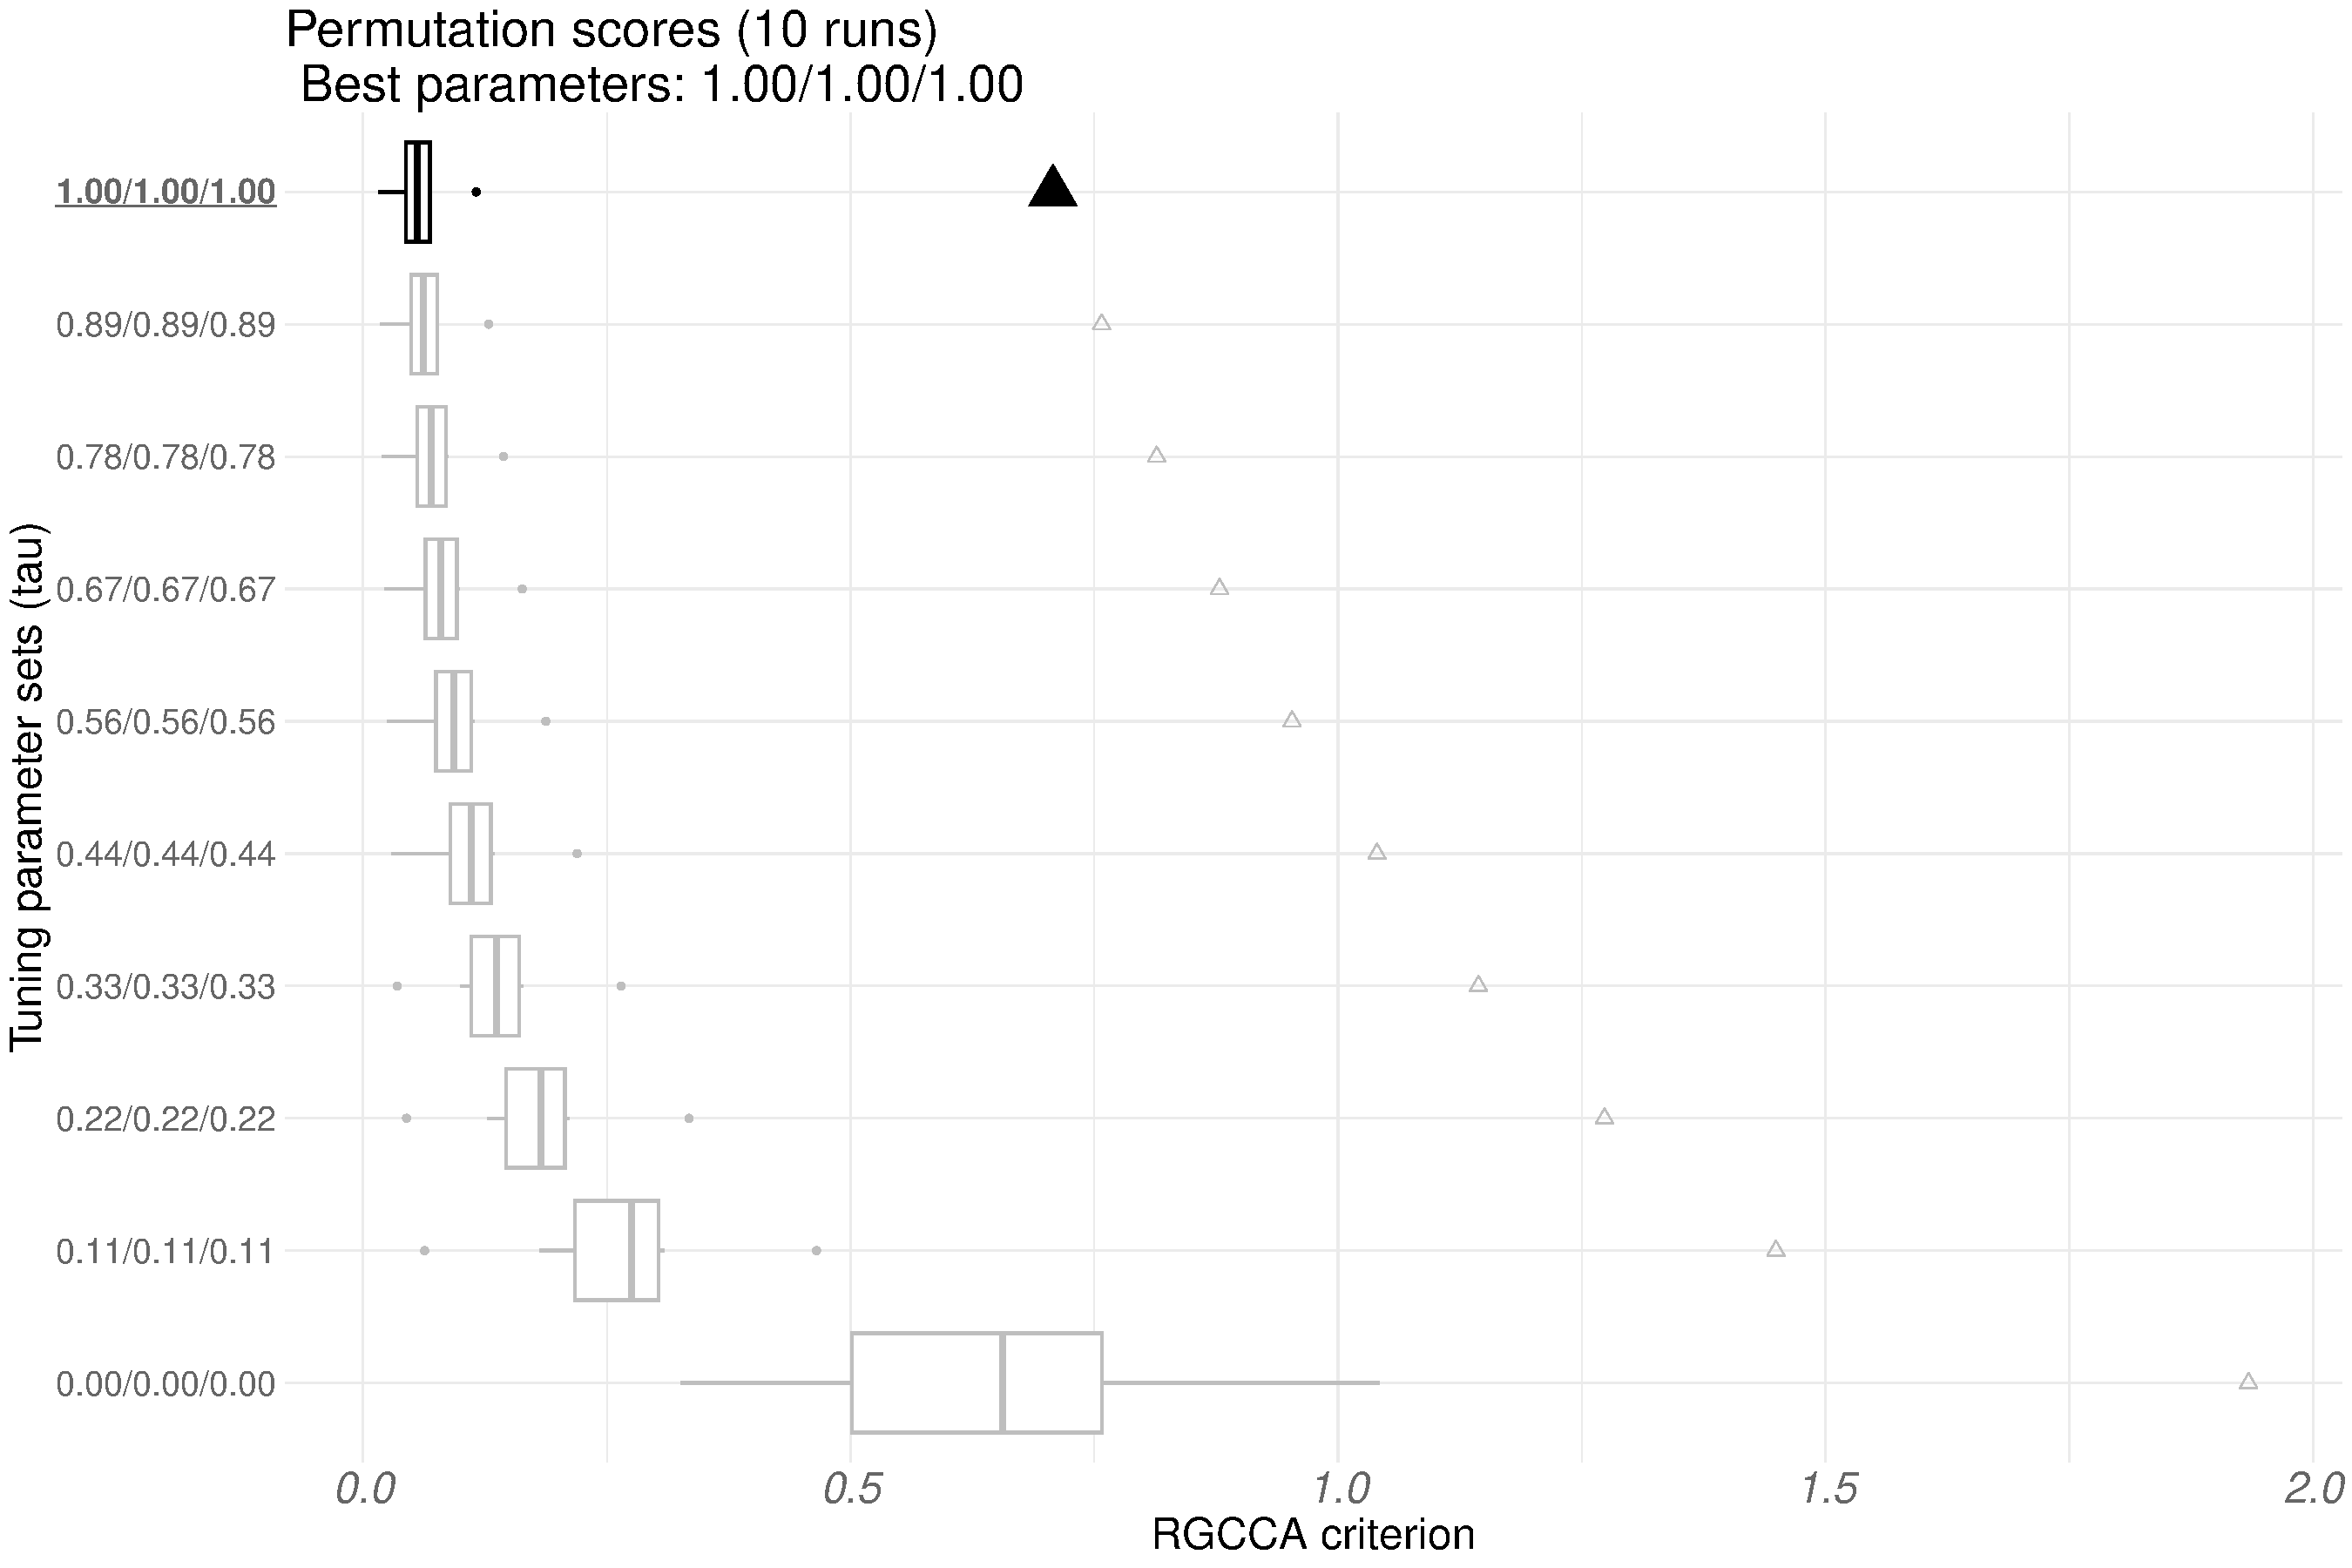
\includegraphics{figures/unnamed-chunk-23-1} 

}

\caption[Values of the objective function of RGCCA against the sets of tuning parameters, triangles correspond to evaluations on non-permuted datasets]{Values of the objective function of RGCCA against the sets of tuning parameters, triangles correspond to evaluations on non-permuted datasets.}\label{fig:unnamed-chunk-23}
\end{figure}
\end{CodeChunk}

\normalsize

The fitted permutation object, \(\small{\texttt{perm\_out}}\), can be
directly provided as the output of \(\small{\texttt{rgcca()}}\) and
visualized/bootstrapped as usual.

\footnotesize

\begin{CodeChunk}
\begin{CodeInput}
R> fit <- rgcca(perm_out)
\end{CodeInput}
\end{CodeChunk}

\normalsize

Of course, it is possible to define explicitly the combination of
regularization parameters to be tested. In that case, a matrix of
dimension \(K \times J\) is required. Each row of this matrix
corresponds to one set of tuning parameters. Alternatively, a numeric
vector of length \(J\) indicating the maximum range values to be tested
can be given. The set of parameters is then uniformly generated between
the minimum values (0 for RGCCA and \(1/\text{sqrt}(\text{ncol})\) for
SGCCA) and the maximum values specified by the user with
\(\small{\texttt{par\_value}}\).

\textbf{Cross-validation strategy.} The optimal tuning parameters can
also be obtained by cross-validation. We will illustrate this in the
next section in the context of SGCCA.

\hypertarget{high-dimensional-case-study-glioma-data}{%
\section{High dimensional case study: Glioma
Data}\label{high-dimensional-case-study-glioma-data}}

\textbf{Biological problem.} Brain tumors are children's most common
solid tumors and have the highest mortality rate of all pediatric
cancers. Despite advances in multimodality therapy, children with pHGG
invariably have an overall survival of around 20\% at 5 years. Depending
on their location (e.g.~brainstem, central nuclei, or supratentorial),
pHGG present different characteristics in terms of radiological
appearance, histology, and prognosis. Our hypothesis is that pHGG have
different genetic origins and oncogenic pathways depending on their
location. Thus, the biological processes involved in the development of
the tumor may be different from one location to another, as has been
frequently suggested.

\textbf{Description of the data.} Pretreatment frozen tumor samples were
obtained from 53 children with newly diagnosed pHGG from Necker Enfants
Malades (Paris, France) \citep{Puget2012}. The 53 tumors are divided
into 3 locations: supratentorial (HEMI), central nuclei (MIDL), and
brain stem (DIPG). The final dataset is organized into 3 blocks of
variables defined for the 53 tumors: the first block \(\mathbf{X}_1\)
provides the expression of \(15702\) genes (GE). The second block
\(\mathbf{X}_2\) contains the imbalances of \(1229\) segments (CGH) of
chromosomes. \(\mathbf{X}_3\) is a block of dummy variables describing
the categorical variable location. One dummy variable has been left out
because of redundancy with the others.

The next lines of code can be run to download the dataset:

\footnotesize

\begin{CodeChunk}
\begin{CodeInput}
R> # Download the dataset's package at http://biodev.cea.fr/sgcca/.
R> # --> gliomaData_0.4.tar.gz
R> if (!("gliomaData" %in% rownames(installed.packages()))) {
+   destfile <- tempfile()
+   download.file("http://biodev.cea.fr/sgcca/gliomaData_0.4.tar.gz", destfile)
+   install.packages(destfile, repos = NULL, type = "source")
+ }
\end{CodeInput}
\end{CodeChunk}

\normalsize

\footnotesize

\begin{CodeChunk}
\begin{CodeInput}
R> data(ge_cgh_locIGR, package = "gliomaData")
R> 
R> blocks <- ge_cgh_locIGR$multiblocks
R> Loc <- factor(ge_cgh_locIGR$y)
R> levels(Loc) <- colnames(ge_cgh_locIGR$multiblocks$y)
R> blocks[[3]] <- Loc
R> 
R> # check dimensions of the blocks
R> vapply(blocks, NCOL, FUN.VALUE = 1L)
\end{CodeInput}
\end{CodeChunk}

\normalsize

We impose \(\mathbf{X}_1\) and \(\mathbf{X}_2\) to be connected to
\(\mathbf{X}_3\). This design is commonly used in many applications and
is oriented toward predicting the location. The argument
\(\small{\texttt{response = 3}}\) of the \(\small{\texttt{rgcca()}}\)
function encodes this design.

\footnotesize

\begin{CodeChunk}
\begin{CodeInput}
R> fit.rgcca <- rgcca(blocks = blocks, response = 3, ncomp = 2, verbose = FALSE)
\end{CodeInput}
\end{CodeChunk}

\normalsize

When the response variable is qualitative, two steps are implicitly
performed: (i) disjunctive coding and (ii) the associated shrinkage
parameter is set to \(0\) regardless of the value specified by the user.

\footnotesize

\begin{CodeChunk}
\begin{CodeInput}
R> fit.rgcca$call$connection
R> fit.rgcca$call$tau
\end{CodeInput}
\end{CodeChunk}

\normalsize

From the dimension of each block (\(n>p\) or \(n\leq p\)),
\(\small{\texttt{rgcca()}}\) selects automatically the dual formulation
for \(\mathbf{X}_1\) and \(\mathbf{X}_2\) and the primal one for
\(\mathbf{X}_3\). The formulation used for each block is returned using
the following command:

\footnotesize

\begin{CodeChunk}
\begin{CodeInput}
R> fit.rgcca$primal_dual
\end{CodeInput}
\end{CodeChunk}

\normalsize

The dual formulation makes the RGCCA algorithm highly efficient, even in
a high-dimensional setting.

\footnotesize

\begin{CodeChunk}
\begin{CodeInput}
R> system.time(
+   rgcca(blocks = blocks, response = 3)
+ )
\end{CodeInput}
\end{CodeChunk}

\normalsize

RGCCA enables visual inspection of the spatial relationships between
classes. This facilitates assessment of the quality of the
classification and makes it possible to determine which components
capture the discriminant information readily.

\footnotesize

\begin{CodeChunk}
\begin{CodeInput}
R> plot(fit.rgcca, type = "sample", block = 1:2,
+      comp = 1, response = Loc, cex = 2)
\end{CodeInput}
\end{CodeChunk}

\normalsize

For easier interpretation of the results, especially in high-dimensional
settings, it is often appropriate to add penalties promoting sparsity
within the RGCCA optimization problem. For that purpose, an \(\ell_1\)
penalization on the weight vectors
\(\mathbf{a}_1, \ldots, \mathbf{a}_J\) is applied. the
\(\small{\texttt{sparsity}}\) argument of \(\small{\texttt{rgcca()}}\)
varies between 1/sqrt(ncol) and 1 (larger values of
\(\small{\texttt{sparsity}}\) correspond to less penalization) and
controls the amount of sparsity of the weight vectors
\(\mathbf{a}_1, \ldots, \mathbf{a}_J\). If \(\small{\texttt{sparsity}}\)
is a vector, \(\ell_1\)-penalties are the same for all the weights
corresponding to the same block but different components:

\begin{equation}
\forall h, \Vert \mathbf{a}_j^{(h)} \Vert_{\ell_1} \leq \small{\texttt{sparsity}}_j \sqrt{p_j},
\end{equation}

with \(p_j\) the number of variables of \(\mathbf X_j\).

If \(\small{\texttt{sparsity}}\) is a matrix, row \(h\) of
\(\small{\texttt{sparsity}}\) defines the constraints applied to the
weights corresponding to components \(h\):

\begin{equation}
\forall h, \Vert \mathbf{a}_j^{(h)} \Vert_{\ell_1} \leq \small{\texttt{sparsity}}_{h,j} \sqrt{p_j}.
\end{equation}

\hypertarget{sgcca-for-the-glioma-dataset}{%
\subsection{SGCCA for the Glioma
dataset}\label{sgcca-for-the-glioma-dataset}}

The algorithm associated with the optimization problem
(\ref{optim_SGCCA}) is available through the function
\(\small{\texttt{rgcca()}}\) with the argument
\(\small{\texttt{method = "sgcca"}}\).

\footnotesize

\begin{CodeChunk}
\begin{CodeInput}
R> fit.sgcca <- rgcca(blocks = blocks, response = 3, ncomp = 2,
+                    sparsity = c(0.0710, 0.2000, 1),
+                    verbose = FALSE)
\end{CodeInput}
\end{CodeChunk}

\normalsize

The \(\small{\texttt{print()}}\) function allows summarizing the SGCCA
analysis,

\footnotesize

\begin{CodeChunk}
\begin{CodeInput}
R> print(fit.sgcca)
\end{CodeInput}
\end{CodeChunk}

\normalsize

and the \(\small{\texttt{plot()}}\) returns the same graphical displays
as RGCCA. We skip these representations for sake of brevity.

Of course, it is still possible to determine the optimal sparsity
parameters by permutation. This is made possible by setting the
\(\small{\texttt{par\_type}}\) argument to
\(\small{\texttt{"sparsity"}}\) (instead of \(\small{\texttt{"tau"}}\))
within the \(\small{\texttt{rgcca\_permutation()}}\) function. However,
we will use another approach in this section.

\textbf{Cross-validation strategy.} The optimal tuning parameters can be
determined by cross-validating different indicators of quality, namely:

\begin{itemize}
\item
  For classification: \(\small{\texttt{Accuracy}}\),
  \(\small{\texttt{Kappa}}\), \(\small{\texttt{F1}}\),
  \(\small{\texttt{Sensitivity}}\), \(\small{\texttt{Specificity}}\),
  \(\small{\texttt{Pos\_Pred\_Value}}\),
  \(\small{\texttt{Neg\_Pred\_Value}}\), \(\small{\texttt{Precision}}\),
  \(\small{\texttt{Recall}}\), \(\small{\texttt{Detection\_Rate}}\), and
  \(\small{\texttt{Balanced\_Accuracy}}\).
\item
  For regression: \(\small{\texttt{RMSE}}\) and
  \(\small{\texttt{MAE}}\).
\end{itemize}

This cross-validation protocol is made available through the
\(\small{\texttt{rgcca\_cv}}\) function and is used here for predicting
the location of the tumors.

In this situation, the goal is to maximize the cross-validated accuracy
(\(\small{\texttt{metric = "Accuracy"}}\)) in a model where we try to
predict the response block from all the block components with a
user-defined classifier
(\(\small{\texttt{prediction\_model = "lda"}}\)). Also, we decide to
upper bound the sparsity parameters for \(\mathbf X_1\) and
\(\mathbf X_2\) to \(0.2\) to achieve an attractive amount of sparsity.

\footnotesize

\begin{CodeChunk}
\begin{CodeInput}
R> set.seed(27) #my favorite number
R> inTraining <- caret::createDataPartition(
+   blocks[[3]], p = .75, list = FALSE
+ )
R> training <- lapply(blocks, function(x) as.matrix(x)[inTraining, , drop = FALSE])
R> testing <- lapply(blocks, function(x) as.matrix(x)[-inTraining, , drop = FALSE])
R> 
R> cv_out <- rgcca_cv(blocks = training, response = 3,
+                    par_type = "sparsity",
+                    par_value = c(.2, .2, 0),
+                    par_length = 10,
+                    prediction_model = "lda",
+                    validation = "kfold",
+                    k = 3, n_run = 5, metric = "Accuracy",
+                    n_cores = 2)
\end{CodeInput}
\end{CodeChunk}

\normalsize

\(\small{\texttt{rgcca\_cv()}}\) relies on the
\(\small{\texttt{caret}}\) package. As a direct consequence, an
astonishingly large number of models are made available (see
\(\small{\texttt{caret::modelLookup()}}\)). Results of the
cross-validation procedure are reported using the generic
\(\small{\texttt{print()}}\) function,

\footnotesize

\begin{CodeChunk}
\begin{CodeInput}
R> print(cv_out)
\end{CodeInput}
\end{CodeChunk}

\normalsize

and displayed using the generic \(\small{\texttt{plot()}}\) function.

\footnotesize

\begin{CodeChunk}
\begin{CodeInput}
R> plot(cv_out, cex = 2)
\end{CodeInput}
\end{CodeChunk}

\normalsize

As previously, the optimal sparsity parameters can be used to fit a new
model, and the resulting optimal model can be visualized/bootstrapped.

\footnotesize

\begin{CodeChunk}
\begin{CodeInput}
R> fit <- rgcca(cv_out)
R> print(fit)
\end{CodeInput}
\end{CodeChunk}

\normalsize

Note that the sparsity parameter associated with \(\mathbf{X}_3\)
switches automatically to \(\tau_3 = 0\). This choice is justified by
the fact that we were not looking for a block component \(\mathbf y_3\)
that explained its own block well (since \(\mathbf{X}_3\) is a group
coding matrix) but one that is correlated with its neighboring
components.

At last, \(\small{\texttt{rgcca\_predict()}}\) can be used for
predicting new blocks,

\footnotesize

\begin{CodeChunk}
\begin{CodeInput}
R> pred <- rgcca_predict(fit, blocks_test = testing, prediction_model = "lda")
\end{CodeInput}
\end{CodeChunk}

\normalsize

and a \(\small{\texttt{caret}}\) summary of the performances can be
reported.

\footnotesize

\begin{CodeChunk}
\begin{CodeInput}
R> pred$confusion$test
\end{CodeInput}
\end{CodeChunk}

\normalsize

If, for a specific reason, only the block components are wanted for the
test set, the function \(\small{\texttt{rgcca\_transform}}\) can be
used.

\footnotesize

\begin{CodeChunk}
\begin{CodeInput}
R> projection <- rgcca_transform(fit, blocks_test = testing)
\end{CodeInput}
\end{CodeChunk}

\normalsize

\textbf{Stability procedure.} It is possible to stabilize the selected
variables using the following procedure.

\cite{Tenenhaus1998} defines the Variable Importance in Projection (VIP)
score for the PLS method. This score is used for variable selection: the
higher the score, the more important the variable. We use this idea to
propose a procedure for evaluating the stability of the variable
selection procedure of SGCCA. This procedure relies on the following
score:

\begin{equation}
\displaystyle \mathrm{VIP}(\mathbf{x}_{jh}) = \frac{1}{K} \sum_{k=1}^K \left(\mathbf{a}_{jh}^{(k)2} \mathrm{AVE}\left(\mathbf X_j^{(k)}\right)\right).
\label{VIP}
\end{equation}

SGCCA is run several times using a bootstrap resampling procedure. For
each model, the VIPs are computed, and the variables with the higher
VIPs averaged over the different models are kept. This procedure is
available through the \(\small{\texttt{rgcca\_stability}}\) function.

\footnotesize

\begin{CodeChunk}
\begin{CodeInput}
R> fit_stab <- rgcca_stability(fit,
+                             keep = vapply(
+                               fit$a, function(x) mean(x != 0),
+                               FUN.VALUE = 1.0
+                             ),
+                             n_boot = 100, verbose = TRUE, n_cores = 2)
\end{CodeInput}
\end{CodeChunk}

\normalsize

Once the most stable variables have been found, a new model using these
variables is automatically fitted. This last model can be visualized
using the usual \(\small{\texttt{print()}}\) and
\(\small{\texttt{plot()}}\) functions.

\footnotesize

\begin{CodeChunk}
\begin{CodeInput}
R> plot(fit_stab, type = "sample", block = 1:2,
+      comp = 1, resp = as.character(Loc)[inTraining],
+      cex = 2
+      )
\end{CodeInput}
\end{CodeChunk}

\normalsize

We can finally apply the bootstrap procedure on the most stable
variables.

\footnotesize

\begin{CodeChunk}
\begin{CodeInput}
R> boot_out <- rgcca_bootstrap(fit_stab, n_boot = 500)
\end{CodeInput}
\end{CodeChunk}

\normalsize

The bootstrap results can be visualized using the generic
\(\small{\texttt{plot()}}\) function. We use the
\(\small{\texttt{n\_mark}}\) parameter to display the top 50 variables
of GE.

\footnotesize

\begin{CodeChunk}
\begin{CodeInput}
R> plot(boot_out, block = 1,
+      display_order = FALSE,
+      n_mark = 50, cex = 1.5, cex_sub = 17,
+      show_star = TRUE)
\end{CodeInput}
\end{CodeChunk}

\normalsize

\hypertarget{conclusion}{%
\section{Conclusion}\label{conclusion}}

The RGCCA framework gathers fifty years of multiblock component methods
and offers a unified implementation strategy for these methods. The
RGCCA package is available on the Comprehensive R Archive Network (CRAN)
and GitHub \url{https://github.com/rgcca-factory/RGCCA}. This release of
the RGCCA package includes:

\begin{itemize}
\item Several strategies for determining the shrinkage 
parameters/level of sparsity automatically: Schaffer \& Strimmer's analytical formulae, 
cross-validation, or permutation strategy.

\item A bootstrap resampling procedure for assessing the reliability of the 
parameter estimates of S/RGCCA.

\item Dedicated functions for graphical displays of the output of RGCCA 
(sample plot, correlation circle, biplot, ...).

\item Various implementation strategies for orthogonal block-components or 
orthogonal block-weight vectors.


\item Strategies for handling missing data. Specifically, multiblock data 
faces two types of missing data structure: (i) if an 
observation $i$ has missing values on a whole block j and (ii) if an 
observation i has some missing values on a block j (but not all). For these two 
situations, we exploit the algorithmic solution proposed for PLS 
path modeling to deal with missing data \citep[see][]{Tenenhaus2005}.

\item Special attention has been paid to providing a bunch of "mathematical" unit tests 
which, in a sense, guarantee the implementation quality. Also, when appropriate, a particular focus was given to recovering the results of other R packages of the literature , including $\small{\texttt{ade4}}$ and $\small{\texttt{FactoMineR}}$.
\end{itemize}

We believe that the RGCCA package will be a valuable resource for
researchers and practitioners who are interested in multiblock data
analysis to gain new insights and improve decision-making.

The RGCCA framework is constantly evolving and extending. Indeed, we
proposed RGCCA for multigroup data \citep{Tenenhaus2014b}, RGCCA for
multiway data \citep{Gloaguen2020, Girka2023} and RGCCA for (sparse and
irregular) functional data \citep{Sort2023}. In addition, maximizing
successive criteria may be seen as sub-optimal from an optimization
point of view, where a single global criterion might be preferred. A
global version of RGCCA \citep{Gloaguen2020b}, which allows
simultaneously extracting several components per block (no deflation
procedure required), has been proposed. Also, it is possible to use
RGCCA in structural equation modeling with latent and emergent variables
for obtaining consistent and asymptotically normal estimators of the
parameters \citep{Tenenhaus2023}. At last, several alternatives for
handling missing values are discussed in \cite{Peltier2022}. Work in
progress includes the integration of all these novel approaches in the
next release of the RGCCA package.

\hypertarget{acknowledgments}{%
\section*{Acknowledgments}\label{acknowledgments}}
\addcontentsline{toc}{section}{Acknowledgments}

This project has received funding from UDOPIA - ANR-20-THIA-0013, the
European Union's Horizon 2020 research and innovation program under
grant agreement No 874583 and the AP-HP Foundation, within the framework
of the AIRACLES Chair.

\renewcommand\refname{References}
\bibliography{biblio.bib}



\end{document}
